\chapter{Asynchronous Rumour Spreading}
\label{chapter:AsyncUpperBound}

In this chapter we introduce the dynamic network model and define an algorithm for rumour spreading on this model introduced by Pourmiri and Mans in \cite{asyncPaper}. We then prove a bound from \cite{asyncPaper} on the associated spreading time that holds w.h.p. We conclude the chapter by investigating how useful this bound is in practice. We apply the bound to a selection of simple dynamic networks, and compare the results with simulated spreading times. 

\section{The Dynamic Network Model}

Here we formally define the Dynamic Network structure on which rumours will spread.

\begin{definition}
	Dynamic Network

	\noindent
	A dynamic network is a sequence of graphs $\mathcal{G} = (G_t)_{t \geq 0}$ indexed by an integer time $t$. All the graphs in the sequence have the same vertex set at each time step, but the edge set may vary, i.e.  $G_t = (V, E_t)$ where $E_t$ is some edge set on $V$.
\end{definition}

$G_t$ represents the topology of the network at the discrete time step $t$. However, asynchronous rumour spreading algorithms operate in continuous time, so we need to define the topology of the network at non-integer times. To represent the state of the network at a continuous time $\gamma \geq 0$, we say that $G_\gamma$ := $G_{\floor\gamma}$. Thus, for any time $\gamma \in [t, t + 1)$ the network topology is fixed to $G_t$. Hence, the topology of the network can only change at integer time steps.

We also need to adjust some of the notation introduced in Section \ref{section:graphNotation} to accommodate for the changes in the network topology over time.

\begin{definition}
	Vertex degree at time $\gamma \in \mathbb{R}_+ $ 

	\noindent
	For a Dynamic Network $\mathcal{G}$ on a vertex set $V$, $d_v(\gamma)$ is the degree of a vertex $v \in V$ at time $\gamma$, i.e. the degree of $v$ in $G_\gamma$
\end{definition}

\begin{definition}
	Dynamic Network Isomorphism

	We say that two dynamic networks $\mathcal{G}_1 = (G_t)_{t \geq 0}$ and $\mathcal{G}_2 = (H_t)_{t \geq 0}$ are isomorphic if the topologies $G_t$ and $H_t$ are isomorphic for all $t \geq 0$. 
\end{definition}

\section{The Asynchronous Rumour Spreading Model}

We are ready to define our first asynchronous algorithm for rumour spreading on a dynamic network.

\begin{definition}
	Asynchronous Push-Pull Rumour Spreading Algorithm for Dynamic Networks
\end{definition}
\label{NodeCentricAsyncAlgorithm}

\noindent
An asynchronous rumour spreads on a given dynamic network $\mathcal{G} = (G_t)_{t \geq 0}$ in rounds, each lasting a unit length of time. Initially a single node is aware of the rumour. In round $t$, the rumour spreads according to the Asynchronous Push-Pull Rumour Spreading Algorithm for Static Topologies (Algorithm \ref{algo:staticAsync}) on the topology $G_t$.

We take a moment to consider the implications of the changes this model introduces. We observed that in the static network algorithm, the random set of active edges is dependent on the state of the network. However, the dynamic model introduces an additional layer of complexity, as the set of active edges also depends on the current topology, and hence on the time. Thus, the spreading time random variable is dependent on when spreading events occur, in addition to which nodes were involved. This dependence introduces further complexity into the spreading time analysis.

% An interesting observation is that unlike the static model, in Algorithm \ref{NodeCentricAsyncAlgorithm} the spreading time 
% P1 MAYBE: allows for topologies to be discconnected with finite spreading time - probability that spreadin time infinite - taken care of by bound

\section{Bounding the Spreading Times}

We follow a proof of an upper bound on the spreading times of this model for an arbitrary network by Pourmiri and Mans \cite{asyncPaper}. We explain steps in greater detail than in the original paper.

First we prove a lemma about how long it takes for the number of nodes aware of the rumour to increase by a multiplicative factor. 

\begin{lemma} \label{AsyncIncreaseLemma}
	Let $\mathcal{G}=(G_t)_{t \geq 0}$ be an $n$-node dynamic network. At $t=0$ a single node is aware of rumour which spreads according to Algorithm \ref{NodeCentricAsyncAlgorithm}. Choose an arbitrary time $\tau \in [0, \infty)$.
	\noindent
	Define 
	
	$$
	\Delta_\tau(\alpha) = \min \left\{t: \sum_{k=0}^t \Phi(G_{\ceil*{\tau}+k})\rho(G_{\ceil*{\tau}+k}) \geq 2 \alpha \right\}
	$$

	\noindent
	Let $\tau'$ denote the earliest time when $|I_t|$ increases by $\frac{m(\tau)}{2}$, where $m(\tau) := \min\{|I_\tau|, |U_\tau|\}$, i.e,
	$$
		\tau' = \min\left\{\gamma : |I_{\gamma}| \geq |I_\tau| + \frac{m(\tau)}{2}\right\}
	$$
	\noindent
	Then, 
	$$
		\mathbb{P}(\tau' - \tau \geq \Delta_\tau(\alpha) + 2) \leq e^{-c_0\alpha m(\tau)}
	$$
	\noindent
	where $c_0 = \frac{1}{2} - \frac{\log 2}{2}$
\end{lemma}

At first sight, it may be difficult to identify the relationship that this lemma expresses, so we first explore the implications of the result, before moving to the proof.

When less than half of the nodes are aware of the rumour, we can interpret $\tau'$ as the first time at which the number of informed nodes increases by a half, compared to number of informed nodes at time $\tau$. In this case $|I_{\tau'}| \approxeq \frac{3}{2} |I_\tau|$. When more than half of the nodes are informed, $\tau'$ is the first time at which the set of uniformed nodes shrinks in size by a half, i.e $|U_{\tau'}| \approxeq \frac{|U_\tau|}{2}$. Thus, the random quantity of interest $\tau'-\tau$ is the amount of time it takes for the number of informed nodes to expand by a multiplicative factor, from time $\tau$. 

In Lemma \ref{AsyncIncreaseLemma} we are interested in the event that this time exceeds $\Delta(\alpha) + 2$. 
The  $+2$ term arises from technicalities in the proof, however the $\Delta_\tau(\alpha)$ term reveals a relationship between to the rate at which the set of informed nodes expands, and the connectivity of the dynamic network.
Suppose we fix $\alpha$ and $\tau$. From the definition of $\Delta_\tau(\alpha)$ we see that the greater the connectivity metrics of the static topologies in the time steps immediately after $\tau$, the smaller the value of $\Delta_\tau(\alpha)$ becomes, since the summation will exceed $2\alpha$ in fewer terms. Thus, we see that well-connected topologies will yield smaller values of $\Delta_\tau(\alpha)$. Returning to the probability bound, we see that the bounding term $e^{-c_0\alpha m(\tau)}$ is independent of the topologies after $\tau$, so the bound has the same probability of failing regardless of the connectivity metrics. Thus, the bound shows that the better the connectivity, the faster the rumour spreads.

\begin{proof}
	Fix $\tau > 0$.
	Fix a time $\gamma \in [\tau, \tau')$. 
	We consider the set of edges $E(I_\gamma, U_\gamma)$ between the informed and uninformed sets of nodes at time $\gamma$. 
	Let $\{u, v\} \in E(I_\gamma, U_\gamma)$ where $u$ is aware of the rumour and $v$ is not.
	Recall that $u$ chooses one of its $d_u(\gamma)$ neighbours uniformly at random to push the rumour to according the arrival times of a unit rate Poisson process. Thus, by the thinning property of Poisson processes, $u$ informs $v$ of the rumour according to the arrival times of a Poisson process with rate $\frac{1}{d_u(\gamma)}$
	Similarly, node $v$ pulls the rumour from one of its $d_v(\gamma)$ neighbours according to a unit rate Poisson process. Thus, $v$ pulls the rumour from $u$ according to a Poisson process of rate $\frac{1}{d_v(\gamma)}$.
	The stochastic process by which $u$ contacts $v$ is the sum of these processes, which itself is a Poisson process with rate $\frac{1}{d_u(\gamma)} + \frac{1}{d_v(\gamma)}$ by the superposition property.
	By considering all the active edges, the cumulative process by which any of the uniformed nodes contact any of the informed nodes is Poisson process of rate 
	$$
	\lambda(\gamma) = \sum_{\{u, v\} \in E(I_\gamma, U_\gamma)} \frac{1}{d_u(\gamma)} + \frac{1}{d_v(\gamma)}
	$$
	by superposition. We note that $\lambda(\gamma)$ is a step function which changes value at the times when the set of active edges changes, i.e, when a new node becomes aware of the rumour or the topology changes. We now derive a lower bound for this rate.
	Let $S = I_\gamma$ if $\text{vol}(I_\gamma) \leq \text{vol}(U_\gamma)$, otherwise let $S = U_\gamma$. Then,

	\begin{align*}
		\lambda(\gamma) &= \sum_{\{u', v'\} \in E(I_\gamma, U_\gamma)} \left\{ \frac{1}{d_{u'}(\gamma)} + \frac{1}{d_{v'}(\gamma)} \right\}\\
		& \geq \sum_{\{u', v'\} \in E(I_\gamma, U_\gamma)}  \max \left\{ \frac{1}{d_{u'}(\gamma)},\frac{1}{d_{v'}(\gamma)} \right\} \\ 
		& \geq \sum_{\{u', v'\} \in E(I_\gamma, U_\gamma)} \min_{\{u, v\} \in E(I_\gamma, U_\gamma) } \left\{ \max \left\{ \frac{1}{d_u(\gamma)},\frac{1}{d_v(\gamma)} \right\} \right\} & \\ 
		\intertext{by replacing all terms in the summation with the minimum term}
		& = \min_{\{u, v\} \in E(I_\gamma, U_\gamma) } 
		\left\{ \max \left\{ \frac{1}{d_u(\gamma)},\frac{1}{d_v(\gamma)} \right\} \right\} |E(I_\gamma, U_\gamma)| \\
		\intertext{since there are  $|E(I_\gamma, U_\gamma)|$ identical terms in the summation}	
		& = \rho(S) \frac{|S|}{\text{vol}(S)} |E(I_\gamma, U_\gamma)| \\
		\intertext{by the definition of $\rho$}
		& = \rho(S) |S| \frac{|E(I_\gamma, U_\gamma)|}{ 
			\min\{\text{vol}(I_\gamma), \text{vol}(U_\gamma)\}
		} \\
		\intertext{by the definition of $S$}
		& \geq \rho(G_\gamma)\Phi(G_\gamma)|S| \\ 
		\intertext{since $\rho$ and $\Phi$ minimise over all valid sets of nodes (including $S$)}
		& \geq \rho(G_\gamma)\Phi(G_\gamma) \min\{|I_\gamma|, |U_\gamma|\} \\
		\intertext{since $S = I_\gamma$ or $ U_\gamma$}
		& = \rho(G_\gamma)\Phi(G_\gamma) m(\gamma)
		\intertext{by the definition of $m(\gamma)$}
	\end{align*}
	We now proceed to prove the following claim, by performing case analysis on $m(\gamma)$

	\textbf{Claim.} $m(\gamma) \geq \frac{m(\tau)}{2}$.

	\textbf{Case 1.} Suppose $m(\gamma) = |I_\gamma|$

	\noindent
	Once a node is aware of the rumour it never becomes uninformed. Hence, as $\tau \leq \gamma$, at time $\gamma$ there are at least $|I_\tau|$ informed nodes, thus 
	$$
	|I_\gamma| \geq |I_\tau| \geq \frac{|I_\tau|}{2} \geq \frac{m(\tau)}{2}
	$$
	so the claim holds in this case.

	\textbf{Case 2.} Suppose instead that $m(\gamma) = |U_\gamma|$

	\noindent
	By the definition of $\tau'$, since $\gamma < \tau'$ we have that $|I_{\gamma}| < |I_\tau| + \frac{m(\tau)}{2}$.

	Since $|I_t| + |U_t| = n$ for all times $t$, note that
	$$
		|I_{\gamma}| < |I_\tau| + \frac{m(\tau)}{2} 
		\iff
		n - |U_{\gamma}| < n - |U_\tau| + \frac{m(\tau)}{2} 
		\iff
		|U_\gamma| > |U_\tau| - \frac{m(\tau)}{2}
	$$
	Thus we have that
	\begin{align*}
		|U_\gamma| & > |U_\tau| - \frac{m(\tau)}{2} & \text{since }\gamma < \tau' \\
		& \geq |U_\tau| - \frac{|U_\tau|}{2} & \text{since } m(\tau) \leq |U_\tau| \\
		& = \frac{|U_\tau|}{2} 
	\end{align*}
	Thus the claim holds in this case also.
	
	\noindent
	By applying the claim to the final inequality in the previous chain of inequalities we get that
	\begin{equation} \label{eq:RateBound}
		\lambda(\gamma) \geq \rho(G_\gamma)\Phi(G_\gamma)\frac{m(\tau)}{2}
	\end{equation}
	So far we have bounded the rate of the Poisson process by which uninformed nodes are made aware of the rumour at time $\gamma$. Since the rate of this transmission process is a function of $\gamma$, we define an inhomogeneous Poisson process $\{N(\gamma), \gamma \geq \tau\}$ with rate function $\lambda(\gamma)$.
	Intuitively, $N(\gamma)$ counts the number of newly informed nodes in the interval $[\tau,\gamma)$. 
	% MAYBE: In actuality, it is a separate process but has the same distribution, defined for a speific realisation, independent of true spread
	Let $\Delta(\alpha)$ denote $\Delta_\tau(\alpha)$ for brevity.
	By the definition of the inhomogeneous Poisson process, $N(\tau + \Delta(\alpha) + 2)$ has a Poisson distribution with rate $\Lambda(\tau + \Delta(\alpha) + 2)$, where
	\begin{align*}
		\Lambda(\tau + \Delta(\alpha) + 2) &= \int_\tau^{\tau + \Delta(\alpha) + 2} \lambda(\gamma) d\gamma \\
		& \geq \int_{\ceil\tau}^{{\ceil\tau} + \Delta(\alpha) + 1} \lambda(\gamma) d\gamma \\
		\intertext{where we note  that $\tau \leq \ceil*{\tau}$ and $\tau > \ceil*{\tau} - 1$, so $[\ceil*{\tau}, {\ceil\tau} + \Delta(\alpha) + 1] \subseteq [\tau, \tau + \Delta(\alpha) + 2]$. Also note that since $\lambda$ is a rate function, $\lambda(\gamma) \geq 0$. Since we integrate over a smaller domain of a non-negative function, the inequality holds.}
		& = \sum_{k=0}^{\Delta(\alpha)} \int_{\ceil\tau + k}^{{\ceil\tau} + k + 1} \lambda(\gamma) d\gamma \\
		\intertext{by splitting the integral into unit length intervals between integers} 
		& \geq \sum_{k=0}^{\Delta(\alpha)} \int_{\ceil\tau + k}^{{\ceil\tau} + k + 1} \rho(G_\gamma)\Phi(G_\gamma)\frac{m(\tau)}{2} d\gamma \\
		\intertext{by applying Inequality \ref{eq:RateBound}}
		& = \sum_{k=0}^{\Delta(\alpha)} \rho(G_{\ceil\tau + k})\Phi(G_{\ceil\tau + k})\frac{m(\tau)}{2} \\
		\intertext{since $G_\gamma = G_{\floor\gamma}$}
		& \geq 2\alpha\frac{m(\tau)}{2} \\
		\intertext{by the definition of $\Delta(\alpha)$}
		& = \alpha m(\tau)
	\end{align*}
	Let $X$ be a random variable with a $\text{Poisson}(\alpha m(\tau))$ distribution. 
	Since $\Lambda(\tau + \Delta(\alpha) + 2) \geq \alpha m(\tau)$, we have that $X$ is first-order stochastically dominated by $N(\tau + \Delta(\alpha) + 2)$ by Theorem \ref{theorem:poissonDomination}.
	Note that
	$$
		\tau' - \tau \geq \Delta(\alpha) + 2 \iff 
		\tau' \geq \tau + \Delta(\alpha) + 2 \implies 
		N(\tau + \Delta(\alpha) + 2) \leq \frac{m(\tau)}{2}
	$$
	where the final implication holds since by the definition of $\tau'$, if $\tau' \geq \tau + \Delta(\alpha) + 2$ then the number of new nodes informed of the rumour between time $\tau$ and $\tau + \Delta(\alpha) + 2$ must be less than or equal to $\frac{m(\tau)}{2}$. Hence, we have that
	\begin{align*}
		\mathbb{P}(\tau' - \tau \geq \Delta(\alpha) + 2) & 
		\leq \mathbb{P}\left(N(\tau + \Delta(\alpha) + 2) \leq \frac{m(\tau)}{2}\right) \\
		& \leq \mathbb{P}\left(X \leq \frac{m(\tau)}{2}\right) \\
		\intertext{since $X$ is stochastically dominated by $N(\tau + \Delta(\alpha) + 2)$} 
		& \leq \mathbb{P}\left(X \leq \frac{\alpha m(\tau)}{2}\right)
		\intertext{since $\alpha \geq 1$}
	\end{align*}
	To finish the proof we prove the following claim

	\noindent
	\textbf{Claim.} For a Poisson($r$) distributed random variable $Y$, 
	$$
		\mathbb{P}(Y \leq \frac{r}{2}) \leq e^{-c_0r}
	$$
	where $c_0$ is the constant defined in the statement of Lemma \ref{AsyncIncreaseLemma}.

	\noindent
	\textit{Proof of Claim}

	\noindent
	From the definition of the density function of Poisson random variables we have that 
	\begin{align*}
		\mathbb{P}(Y \leq \frac{r}{2}) & = e^{-r} \sum_{j=0}^{\floor*{\frac{r}{2}}} \frac{r^j}{j!} \\
		& = e^{-r} \sum_{j=0}^{\floor*{\frac{r}{2}}} \frac{2^j(\frac{r}{2})^j}{j!} \\
		& \leq e^{-r} \sum_{j=0}^{\floor*{\frac{r}{2}}} \frac{2^\frac{r}{2}(\frac{r}{2})^j}{j!} \\
		& \leq e^{-r} e^\frac{r \log 2}{2} \sum_{j=0}^\infty \frac{(\frac{r}{2})^j}{j!} \\
		& \leq e^{-r} e^\frac{r \log 2}{2} e^\frac{r}{2} \\
		& = e^{-c_0r} \\
	\end{align*}
	thus the claim is proved. Since $X \sim \text{Poisson}(\alpha m(\tau))$ we get that
	\begin{align*}
		\mathbb{P}(\tau' - \tau \geq \Delta(\alpha) + 2) \leq \mathbb{P}(X \leq \frac{\alpha m(\tau)}{2}) \leq e^{-c_0 \alpha m(\tau)}
	\end{align*}	
\end{proof}

Now we iteratively apply Lemma \ref{AsyncIncreaseLemma} to derive the following Theorem.

\begin{theorem}\label{theorem:AsyncUpperBound}
	\ModelIntro Let $c \geq 2$ be a constant. Then, with probability $1 - n^{-(c-1)}$, the rumour will have spread to all the nodes of $\mathcal{G}$ in time at most
	$$
		\min \left\{t : \sum_{k=0}^t \Phi(G_k)\rho(G_k) \geq C \log n \right\} 
	$$
	where $C = \lb \frac{2}{\log \frac{3}{2}} + \frac{2}{\log 2} + \frac{12c}{c_0} \rb \log n$
\end{theorem}

\begin{proof}
	We bound the overall spreading time by splitting the rumour spreading in two phases, and bounding lengths of each phase separately.

	\textbf{First Phase.} The first phase starts at time $t=0$ and ends at the first time when the number of informed nodes reaches $\frac{n}{2}$, which we denote $t_\text{half}$. We divide the phase into intervals $[\tau_i, \tau_{i+1}]$ where $\tau_0 = 0$ and $\tau_{i+1}$ is the first time the number of informed nodes increases by $\frac{m(\tau_i)}{2}$. 
	Using the notation from Lemma \ref{AsyncIncreaseLemma}, we have that $\tau_{i+1} = \tau_i'$. 
	
	Note that for all times $\tau < t_\text{half}$, the number of informed nodes is less than $\frac{n}{2}$, so $m(\tau) = |I_\tau|$. Thus, by the following induction at time $\tau_i < t_\text{half}$ there are at least $(\frac{3}{2})^i$ informed nodes.

	\underline{Base Case.}
	By algorithm \ref{NodeCentricAsyncAlgorithm} the rumour spreading starts at time 0 with a single node aware of the rumour. Thus $|I_{\tau_0}| = 1 = (\frac{3}{2})^0$

	\underline{Inductive Case.} 
	Assume that $\tau_i \geq (\frac{3}{2})^i$.
	From the definition of $\tau_i'$, we have that 
	\begin{align*}
		\tau_{i+1} &= \tau_i' \\
		&= \min\left\{\gamma : |I_{\gamma}| \geq |I_{\tau_i}| + \frac{m(\tau_i)}{2}\right\} \\
		&= \min\left\{\gamma : |I_{\gamma}| \geq |I_{\tau_i}| + \frac{|I_{\tau_i}|}{2}\right\} & \text{since } m(\tau_i) = |I_{\tau _i}| \text{ in this phase} \\ 
		&= \min\left\{\gamma : |I_{\gamma}| \geq \frac{3}{2}|I_{\tau_i}|\right\} 
	\end{align*}
	Thus $|I_{\tau_{i+1}}| \geq \frac{3}{2}|I_{\tau_i}| \geq \frac{3}{2}(\frac{3}{2})^i = (\frac{3}{2})^{i+1}$ by the induction hypothesis. 
	
	Let $K$ be the random variable for the index of the final interval in the phase, i.e, the interval where $\tau_K < t_\text{half}$ and $\tau_{K+1} \geq t_\text{half}$.
	Let $N = \ceil*{\log_\frac{3}{2}\frac{n}{2}}$.  Since $|I_{\tau_i}| \geq (\frac{3}{2})^i$, we have that $|I_{\tau_N}| \geq (\frac{3}{2})^N \geq \frac{n}{2}$. Thus, $K < N$ otherwise the number of informed nodes at time $\tau_K$ would be greater than or equal to $\frac{n}{2}$, so $\tau_K$ would be at least $t_\text{half}$ which contradicts the definition of $K$.

	Let $\alpha_i = \ceil*{\frac{c \log n}{c_0 (3/2)^i}}$.
	By Lemma \ref{AsyncIncreaseLemma}, $\Delta(\alpha_i) + 2$ is an upper bound for the length of the interval $[\tau_i, \tau_{i+1}]$ 
	with probability at least $1 - e^{-c_0\alpha_i m(\tau_i)}$ for $i \leq K$.
	Since $m(\tau_i) = |I_{\tau_i}| \geq (\frac{3}{2})^i$, this probability is greater than $1 - e^{-c_0\alpha_i (\frac{3}{2})^i} \geq 1 - e^{-c \log n}$, by the definition of $\alpha_i$. By the union bound over all $K$ intervals of the phase,
	\begin{align*}
		& \mathbb{P}(\text{Any interval has length at least } \Delta_{\tau_i}(\alpha_i) + 2) \\
		&= \mathbb{P}(\bigcup_{i=0}^K \{\tau_{i+1} - \tau_i \geq \Delta_{\tau_i}(\alpha_i) + 2\}) \\
		&\leq \sum_{i=0}^K \mathbb{P}(\tau_{i+1} - \tau_i \geq \Delta_{\tau_i}(\alpha_i) + 2) \\
		\intertext{by the union bound}
		&\leq \sum_{i=0}^K e^{-c \log n} \\
		\intertext{by Lemma \ref{AsyncIncreaseLemma}}	
		&\leq \sum_{i=0}^N e^{-c \log n} \\
		\intertext{since $K < N$}
		&= N n^{-c} \\
		&\leq n^{c-1}
	\end{align*}
	Since $c \geq 2$, w.h.p all intervals have length at least $\Delta(\alpha_i) + 2$, hence
	\begin{equation}\label{eq:t_halfBound}
		t_\text{half} 
		\leq \tau_{K+1} 
		= \sum_{i=0}^K \lb \tau_{i+1} - \tau_i  \rb 
		\leq \sum_{i=0}^K (\Delta_{\tau_i}(\alpha_i) + 2) 
		\leq \sum_{i=0}^N (\Delta_{\tau_i}(\alpha_i) + 2) 
	\end{equation}
	since $K < N$.
	\begin{align*}
		\Delta_{\tau_i}(\alpha_i) + 2 
		&=
		\min \left\{t: \sum_{k=0}^t \Phi(G_{\ceil*{\tau_i}+k})\rho(G_{\ceil*{\tau_i}+k}) \geq 2 \alpha_i \right\} + 2 \\
		&\leq \min \left\{t: \sum_{k=0}^t \Phi(G_{\ceil*{\tau_i}+k})\rho(G_{\ceil*{\tau_i}+k}) \geq 2 \alpha_i + 2 \right\}
	\end{align*}
	since $\Phi(G)\rho(G) \leq 1$ for  any topology $G$. Denote the final expression $\delta_i$. Combining the previous inequalities gives that
	\begin{align*}
		t_\text{half} &\leq \sum_{i=0}^N \min \left\{t: \sum_{k=0}^t \Phi(G_{\ceil*{\tau_i}+k})\rho(G_{\ceil*{\tau_i}+k}) \geq 2 \alpha_i + 2 \right\} = \sum_{i=0}^N \delta_i \\
		&\leq \min \left\{t: \sum_{k=0}^t \Phi(G_k)\rho(G_k) \geq \sum_{i=0}^N (2 \alpha_i + 2) \right\}
	\end{align*}
	We justify the final inequality as follows. Consider the sequence of connectivity metrics $(\Phi(G_k)\rho(G_k))_{k \geq 0}$.
	Note that in the first term, since $\tau_{i+1} \leq \tau_i + \delta_i$, we take sums over potentially overlapping intervals of the sequence of connectivity metrics, namely $[\tau_0, \tau_0 + \delta_0], (\tau_1, \tau_1 + \delta_1], (\tau_2, \tau_2 + \delta_2], \dots$. Thus, each $(\Phi(G_k)\rho(G_k))$ will be considered at least once, and may contribute to multiple terms of the summation due to the overlaps. We can interpret the second sum as iterating in the same way over the following contiguous, disjoint intervals: $[T_0 = 0, T_1 = \Delta_{T_0}(\alpha_0) + 2], (T_1, T_2 = \Delta_{T_1}(\alpha_1) + 2], (T_2, T_3 = \Delta_{T_2}(\alpha_2) + 2], \dots$. Since this sum is taken over disjoint intervals, each $(\Phi(G_k)\rho(G_k))$ term is considered exactly once. Thus, more terms are needed for the contiguous summation $\sum_{k=0}^t \Phi(G_k)\rho(G_k)$ to exceed the sum of the target values $\sum_{i=0}^N (2 \alpha_i + 2)$, since connectivity metrics $\Phi(G_k)\rho(G_k)$ aren't reused.

	Note that in the final bound for $t_\text{half}$ we have eliminated all random quantities such as $\tau_i$ dependent on the rumour spread, thus this bound can be calculated using only information about the network.

	\textbf{Second Phase.} The second phase starts at $t_\text{half}$, when at least $\frac{n}{2}$ nodes have been made aware of the rumour. The phase ends at the first time all nodes are aware of the rumour, which we denote $t_\text{all}$. Note that since the number of informed nodes is at least $\frac{n}{2}$ during this is phase, the number of uninformed nodes is at most $\frac{n}{2}$. Thus, for $\tau > t_\text{half}$, $m(\tau) = |U_\tau|$. From this point, the ideas used to bound the second phase are identical to those in the analysis of the first phase. We omit the analysis of this phase to avoid repetition, and refer the reader to \cite{asyncPaper} for the full details. 

	The result of the second phase analysis is that w.h.p,
	$$
		t_\text{all} - t_\text{half} 
		\leq \min \left\{t: \sum_{k=0}^t \Phi(G_{t_\text{half} +k}) \rho(G_{t_\text{half} +k}) \geq \sum_{j=0}^M (2 \beta_j + 2) \right\}
	$$
	where $\beta_j = \ceil*{\frac{c \log n}{c_0 n(1/2)^j}}$ and $M = \floor*{\log_2 n}$
	By evaluating the geometric sums we have that 
	\begin{align*}
		\sum_{i=0}^N (2 \alpha_i + 2) + \sum_{j=0}^M (2 \beta_j + 2) \leq C
	\end{align*}
	By combining the results from both phases, we have that w.h.p,
	$$
		t_\text{all} = (t_\text{all} - t_\text{half}) + t_\text{half} \leq \min \left\{t : \sum_{k=0}^t \Phi(G_k)\rho(G_k) \geq C \log n \right\} 
	$$
\end{proof}

In Theorem \ref{theorem:AsyncUpperBound}, we have successfully bounded the asynchronous rumour spreading time on dynamic networks. Indeed, using Theorem \ref{theorem:AsyncUpperBound} we can recover the standard result about rumour spreading on static networks from Theorem \ref{theorem:staticBound}. If we let $G_t = G$ for all $t$ (i.e. a static network), by Theorem \ref{theorem:AsyncUpperBound} the rumour spreading time $T$ satisfies 
\begin{align*}
	T &\leq \min \left\{t : \sum_{k=0}^t \Phi(G)\rho(G) \geq C \log n \right\} \\
	&= \min \left\{t : t \Phi(G)\rho(G) \geq C \log n \right\}  \\
	&= \min \left\{t : t \geq \frac{C \log n}{\Phi(G)\rho(G)}\right\}  \\
	&= \mathcal{O}\left(\frac{\log n}{\Phi(G)\rho(G)}\right)
\end{align*}
w.h.p. Encouragingly, we have recovered the same scaling in spreading time as Theorem \ref{theorem:staticBound}.

Theorem \ref{theorem:AsyncUpperBound} also expresses the relationship between the success probability of the bound, and the size of the bound. We recall that the failure probability of the bound is $\mathcal{O}\left(n^{-(c-1)s}\right)$.
We also note that the constant $C$ in Theorem \ref{theorem:AsyncUpperBound} is monotone increasing in $c$. The greater $C$ is, the more terms will be required for the summation to exceed $C \log n$, which will yield a larger bound. 
Thus, the greater the success probability of the bound, the larger the bound will be.

Notice that since the conductance of disconnected topologies is 0, such topologies increase the number of terms needed to exceed $C \log n$ without contributing to the connectivity metric sum. Thus, inserting disconnected topologies into a network increases the spreading time bound, as we would expect. But what happens if all the topologies in the network are disconnected? In this case, the bound is infinite, which tells us no information about the spreading time. However, it is possible for the spreading time to be finite in some such networks, as new edges can enable the rumour to spread between previously disconnected nodes. Consider the network consisting of 3 nodes $\{v_1, v_2, v_3\}$ where only one node knows the rumour initially. Suppose that we alternate between a topology where only $v_1$ and $v_2$ are connected, and a topology where only $v_2$ and $v_3$ are connected. Since all the topologies are disconnected, the bound will be infinite for this network. However, it is almost certain that the rumour will spread to all nodes in a finite time. An interesting avenue for further study is to construct spreading time bounds for networks consisting of disconnected topologies. 
 
% MAYBE: How does diligence affect bound?

\section{Evaluating the quality of the bound}\label{section:asyncEvaluation}

In this section we gauge the quality of the bound given in Theorem \ref{theorem:AsyncUpperBound}, by applying it to various networks, and comparing the results with simulated spreading times.

\subsection{Ring-Complete Alternating Dynamic Network}

First we introduce the dynamic network.

\begin{definition}
	Ring-Complete Alternating Dynamic Network $\mathcal{A}$

	\noindent
	Let $R$ be a graph consisting of a single cycle on $n$ nodes, and $K$ be the complete graph on $n$ nodes. The Ring-Complete Alternating Dynamic Network $\mathcal{A} = (G_t)_{t \geq 0}$ is defined as follows 
	\begin{equation*}
		G_t = 
		\begin{cases*}
			R & if $t = 0 \mod 2$ \\
			K & if $t = 1 \mod 2$
		  \end{cases*}
	\end{equation*}
	i.e. $\mathcal{A}$ alternates between the ring and complete graph topologies.
\end{definition}

Now we apply Theorem \ref{theorem:AsyncUpperBound} to bound the spreading time on the Ring-Complete Alternating Network.

\begin{theorem}\label{theorem:ringCompleteAsyncBound}
	w.h.p the spreading time of Algorithm \ref{NodeCentricAsyncAlgorithm} on the Ring-Complete Alternating Network is at most $\mathcal{O}(\log n)$. 
\end{theorem}

\begin{proof}
By Theorem \ref{theorem:AsyncUpperBound}, w.h.p, the spreading time of the rumour on $\mathcal{A}$ is at most
$$
	\min \left\{t : \sum_{k=0}^t \Phi(G_k)\rho(G_k) \geq C \log n \right\} 
$$
By the definition of $\mathcal{A}$ we have that 
\begin{align*}
	&\min \left\{t : \sum_{k=0}^t \Phi(G_k)\rho(G_k) \geq C \log n \right\} \\
	= &\min \left\{t : \underbrace{\Phi(R)\rho(R) + \Phi(K)\rho(K) + \Phi(R)\rho(R) + \dots}_{t + 1 \text{ terms}} \geq C \log n \right\} \\
	\simeq &\min \left\{t : \frac{t}{2}\Phi(R)\rho(R) + \frac{t}{2}\Phi(K)\rho(K) \geq C \log n \right\} \\
	= &\min \left\{t : t \geq \frac{2C \log n}{\Phi(R)\rho(R) + \Phi(K)\rho(K)} \right\} \\
	= &\ceil*{\frac{2C \log n}{\Phi(R)\rho(R) + \Phi(K)\rho(K)}}
\end{align*}
To calculate this quantity explicitly, we need to compute the conductance and diligence of $R$ and $K$. 

\textbf{Claim 1.} $\Phi(R)=\frac{2}{n}$

We recall from Section \ref{section:graphMetrics} that the definition of conductance for a graph $G$ is 
$$
	\Phi(G) 
	= \min_{\emptyset \neq S \subset V} \frac{|E(S, \comp{S})|}{\min\{\text{vol}(S), \text{vol}(\comp{S})\}} 
$$
We can restrict the domain the minimum optimises over to produce the following equivalent form of the conductance which is easier to work with.
$$
	\Phi(G) 
	= \min_{0 < \text{vol}(S) \leq \frac{\text{vol}(V)}{2}} \frac{|E(S, \comp{S})|}{\text{vol}(S)} 
$$
These expressions are equivalent since for any set $S$ in the original domain, but not the restricted domain, we have that $\text{vol}(S) > \frac{\text{vol}(V)}{2}$, so
$$
	\text{vol}(\comp{S}) 
	= \text{vol}(V) - \text{vol}(S) 
	\leq \frac{\text{vol}(V)}{2}
$$
and since $E(S, \comp{S}) = E(\comp{S}, S)$, we have that
$$
	\frac{|E(S, \comp{S})|}{\min\{\text{vol}(S), \text{vol}(\comp{S})\}} = \frac{|E(\comp{S}, S)|}{\text{vol}(\comp{S})} 
	= 
	\frac{|E(\comp{S}, \comp{\comp{S}})|}{\text{vol}(\comp{S})} 
$$
Thus, for any set of nodes any set $S$ with $\text{vol}(S) > \frac{\text{vol}(V)}{2}$ in the original optimisation domain, we note that the set $\comp{S}$ will be in the restricted optimisation  domain with the same conductance value. Hence, both expressions for the conductance minimise over the same set of conductance values so are equivalent.

Using this simplified definition of the conductance, we can calculate the conductance of the ring graph $R$. 

Let $S \subset V$.  We notice that each set of continuous nodes in $S$ contributes 2 edges between $S$ and $\comp{S}$, one for each endpoint of the contiguous set.
To minimise $|E(S, \comp{S})|$, we take $S$ to be a single contiguous set of $k$ nodes, which yields $|E(S, \comp{S})| = 2$. 

Now we calculate what $k$ should be. Since every node has degree 2, we see that the condition $0 < \text{vol}(S) \leq \frac{\text{vol}(V)}{2}$ is equivalent to the condition $0 < 2k \leq n$, as $\text{vol}(S) = 2|S'|$ for all $S' \subset V$. Hence,
$$
	\Phi(R) 
	=\min_{0 < \text{vol}(S) \leq \frac{\text{vol}(V)}{2}} \frac{|E(S, \comp{S})|}{\text{vol}(S)} 
	= \min_{0 < k \leq \frac{n}{2}} \frac{2}{2k} 
	= \min_{0 < k \leq \frac{n}{2}} \frac{1}{k} 
	= \frac{2}{n}
$$

\textbf{Claim 2.} $\rho(R)=1$

We recall from Section \ref{section:graphMetrics} that the diligence of a subset of nodes $S$ is
$$
\rho(S) = \comp{d}(S) \min_{\{u, v\} \in E(S, \comp{S}) } \left\{ \max \left\{ \frac{1}{d_u},\frac{1}{d_v} \right\} \right\}
$$ 
In $R$ every node has degree 2, so for any node set $S$ the average degree $\comp{d}(S)$ is 2, and 
$$
	\min_{\{u, v\} \in E(S, \comp{S}) } \left\{ \max \left\{ \frac{1}{d_u},\frac{1}{d_v} \right\} \right\}
	= 
	\min_{\{u, v\} \in E(S, \comp{S}) } \left\{ \max \left\{ \frac{1}{2},\frac{1}{2} \right\} \right\}
	=
	\frac{1}{2}
$$
Hence, we obtain $\rho(S) = 2 \frac{1}{2} = 1$ for any $S$. Thus, 
$$
	\rho(R) =  \min_{0 < \text{vol}(S) \leq \frac{\text{vol}(V)}{2}} \rho(S) = 1 
$$
where $V$ denotes the set of $n$ vertices of $R$.

\textbf{Claim 3.}  $\Phi(K)=\frac{1}{2}$

Suppose $S \subset V$ with $|S| = k$. Each of the $k$ nodes in $S$ is connected to all $n - k$ nodes in $\comp{S}$, so $|E(S, \comp{S})| = k(n - k)$. Each node in $S$ is connected to all the remaining $n - 1$ nodes in $V$, so $\text{vol}(S) = k(n-1)$. Since all nodes have the same degree, as in Claim 1, for $K$ the condition that $0 < \text{vol}(S) \leq \frac{\text{vol}(V)}{2}$ is equivalent to the condition that $S$ can consist of at most half the nodes in $K$. Combining the three previous observations together yields that
$$
	\Phi(K) = \min_{0 < \text{vol}(S) \leq \frac{\text{vol}(V)}{2}} \frac{|E(S, \comp{S})|}{\text{vol}(S)} 
	= \min_{0 < k \leq \frac{n}{2}} \frac{k(n-k)}{k(n-1)} 
	= \frac{\frac{n}{2}}{n-1}
	\simeq \frac{1}{2}
$$
for large $n$.

\textbf{Claim 4.}  $\rho(K)=1$

In $K$ every node has degree $n - 1$. Thus, by identical reasoning to Claim 2, we have that for any $S \subseteq V$, $\rho(S) = (n-1)\frac{1}{n-1} = 1$ so $\rho(K) = 1$.

Substituting the values of the connectivity metrics from the previous four claims yields the bound
$$
	\ceil*{\frac{2C \log n}{\Phi(R)\rho(R) + \Phi(K)\rho(K)}} = \ceil*{\frac{2C \log n}{\frac{2}{n} + \frac{1}{2}}}
	= \ceil*{\frac{2n}{4+n} 2C\log n}
	\simeq \ceil*{4C \log n}
$$
for large $n$.

\end{proof}

Recall from Theorem \ref{theorem:staticRingAsyncBound}, that the spreading time also scaled like $\bigO(\log n)$ for the static complete network. Thus, we observe that alternating the complete topology with the low-connectivity ring topology only reduces the speed of the rumour spread by a constant factor.

% MAYBE: how infrequent can high conductance grpah be and still preserve log n scaling? k \in O(1)

Now we compare the bound with simulated spreading times on $\mathcal{A}$.

\begin{figure}[h]
	\centering
	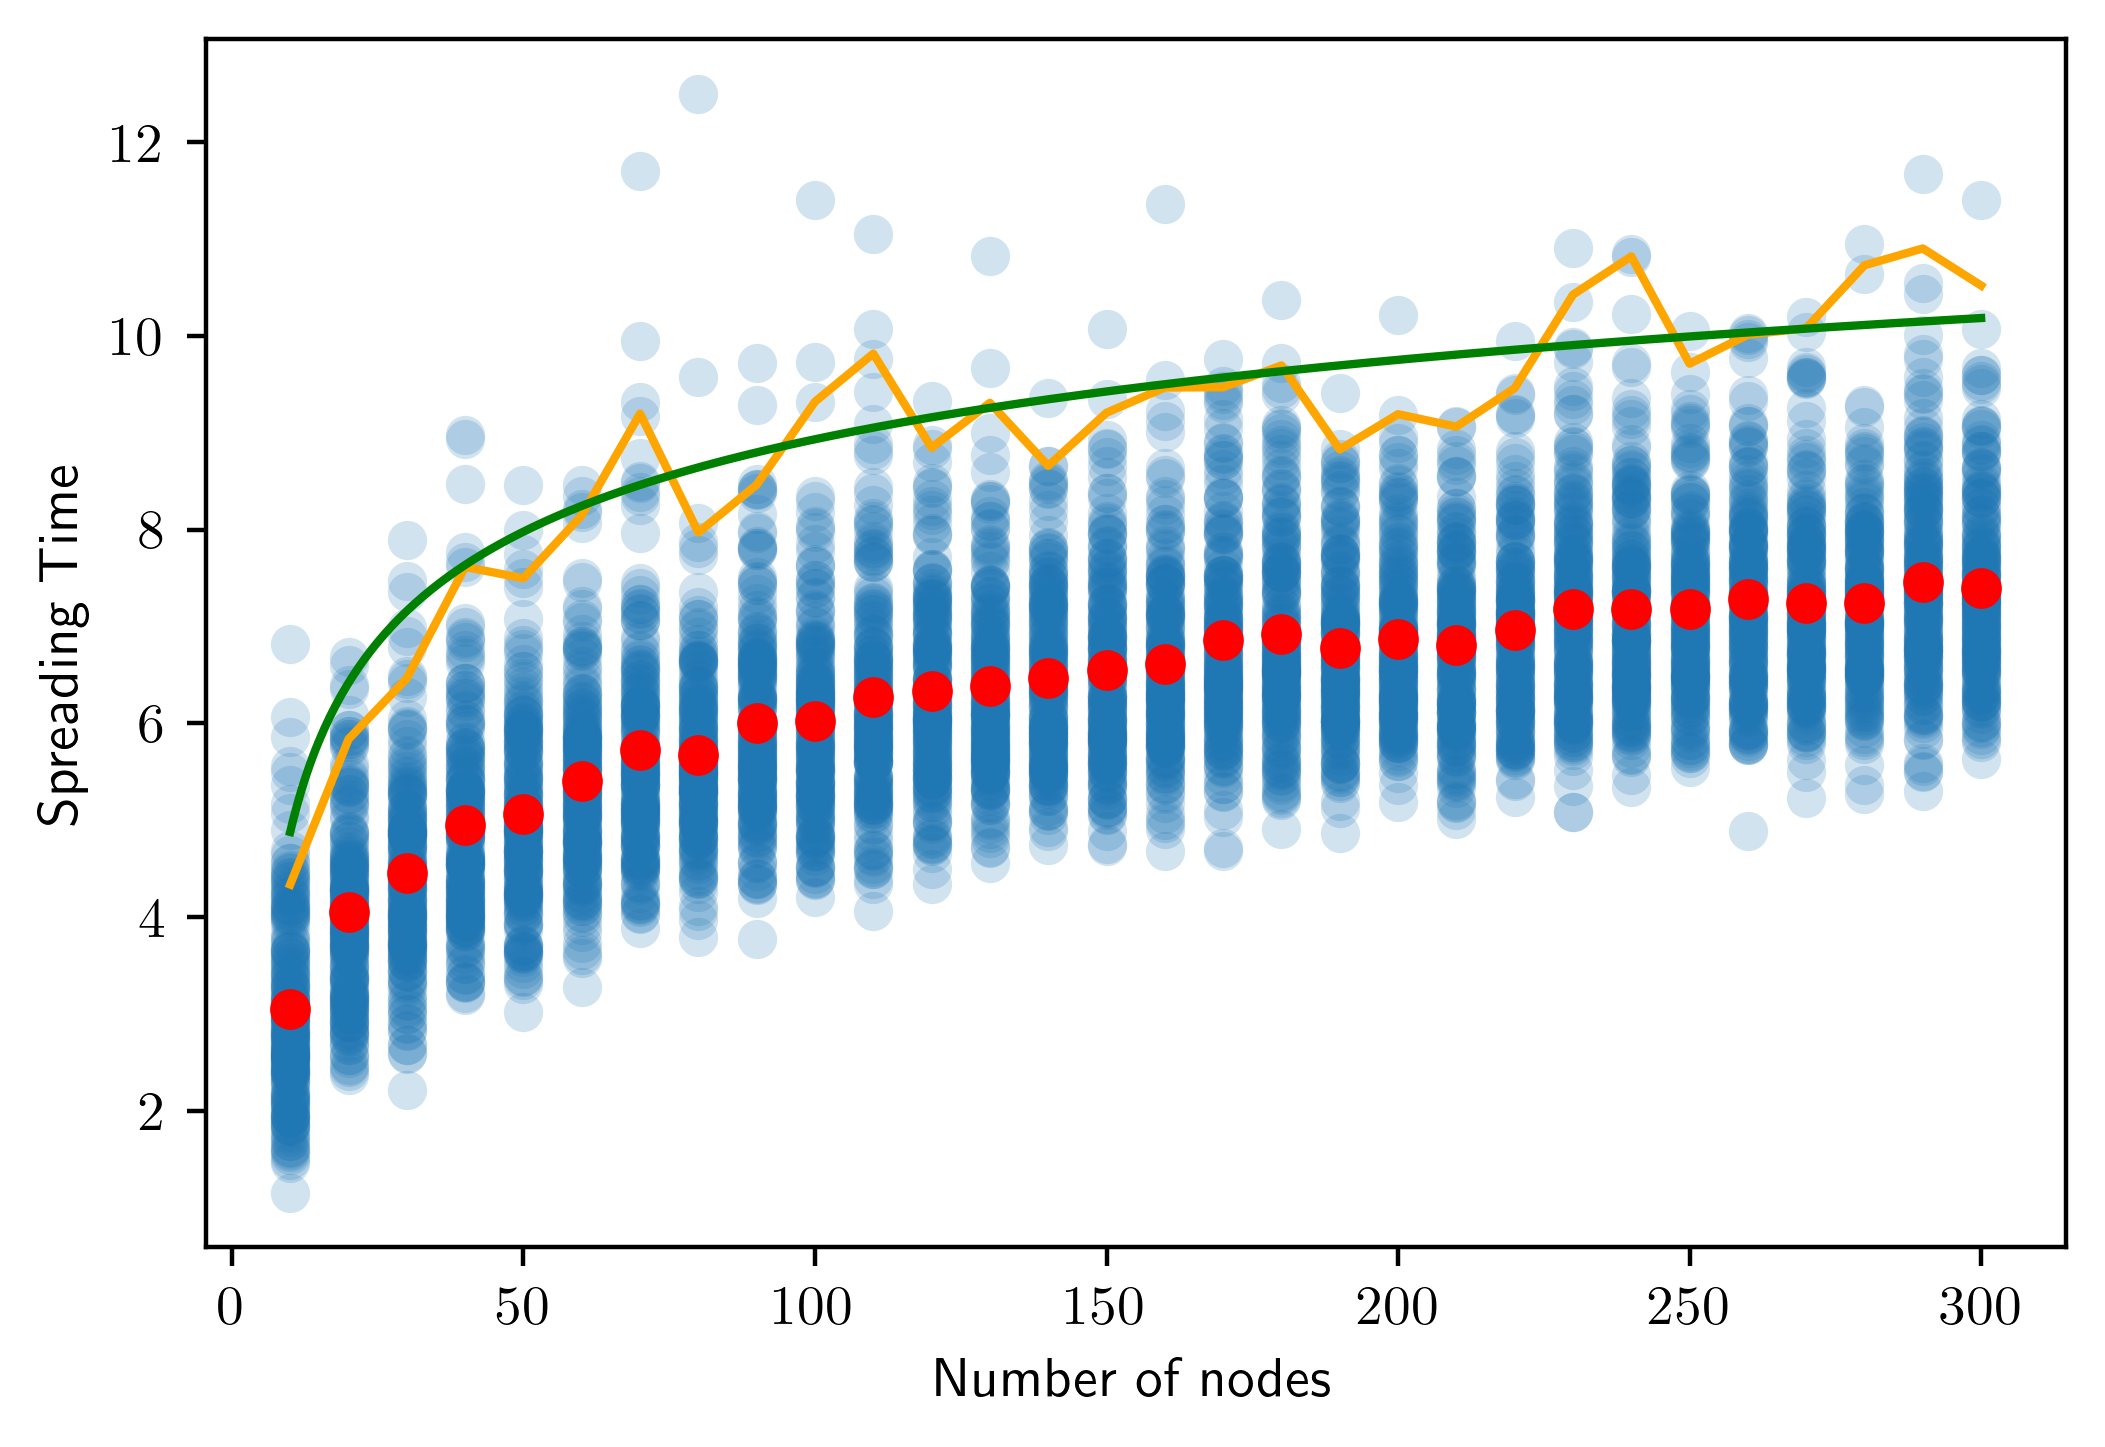
\includegraphics[width=1\textwidth]{./figures/alternating_ring_simulation_results.png}
	\caption{Results of Ring-Complete Alternating Network spreading time simulations}
	\label{fig:alternatingSimResults}
\end{figure}

The scatter plot in Figure \ref{fig:alternatingSimResults} displays the results simulated rumour spreading on $\mathcal{A}$. Each blue point in the plot represents a single simulation, where the $x$ component is the number of nodes in the simulation, and the $y$ component is spreading time. Since the spreading time is random variable, 200 simulations were run for each network size we investigated. The means (displayed by red points) illustrate the relationship between the size of the network and the expected spreading time. 

However, since the bound holds w.h.p, we want to find a value larger than almost all the simulated spreading times for each $n$. Thus, in orange we plot the $99^\text{th}$ percentile of the spreading times for each $n$.

On Figure \ref{fig:floodingGnpSimResultsTight}, we have plotted the function $f(n) = c \log \log (n)$ in green, with an appropriately chosen scaling constant $c$. Note that the $99^\text{th}$ percentile function has a similar growth rate, so these simulations suggest that w.h.p, the spreading time on $\mathcal{A}$ grows like $\mathcal{O}(\log \log n)$ in the network size.

This analysis suggests that the $\mathcal{O}(\log n)$ bound given by Theorem \ref{theorem:AsyncUpperBound} is not tight for $\mathcal{A}$.

Now we evaluate the performance of the bound on another dynamic network.

\subsection{Shuffled Ring}\label{section:shuffledRingAsyncApplication}

We start by introducing the Shuffled Ring Network.

\begin{definition}
	Shuffled Ring Network $\mathcal{S}$

	Let $(G_t)_{t \in \mathbb{N}}$ be the topologies of $\mathcal{S}$. In a shuffled ring network, each $G_t$ is a ring topology (i.e. a single cycle on all the nodes) drawn uniformly at random from the set of all possible ring graphs. 
\end{definition}

\begin{figure}[h]
	\centering
    \begin{subfigure}[b]{0.3\textwidth}
		\centering
		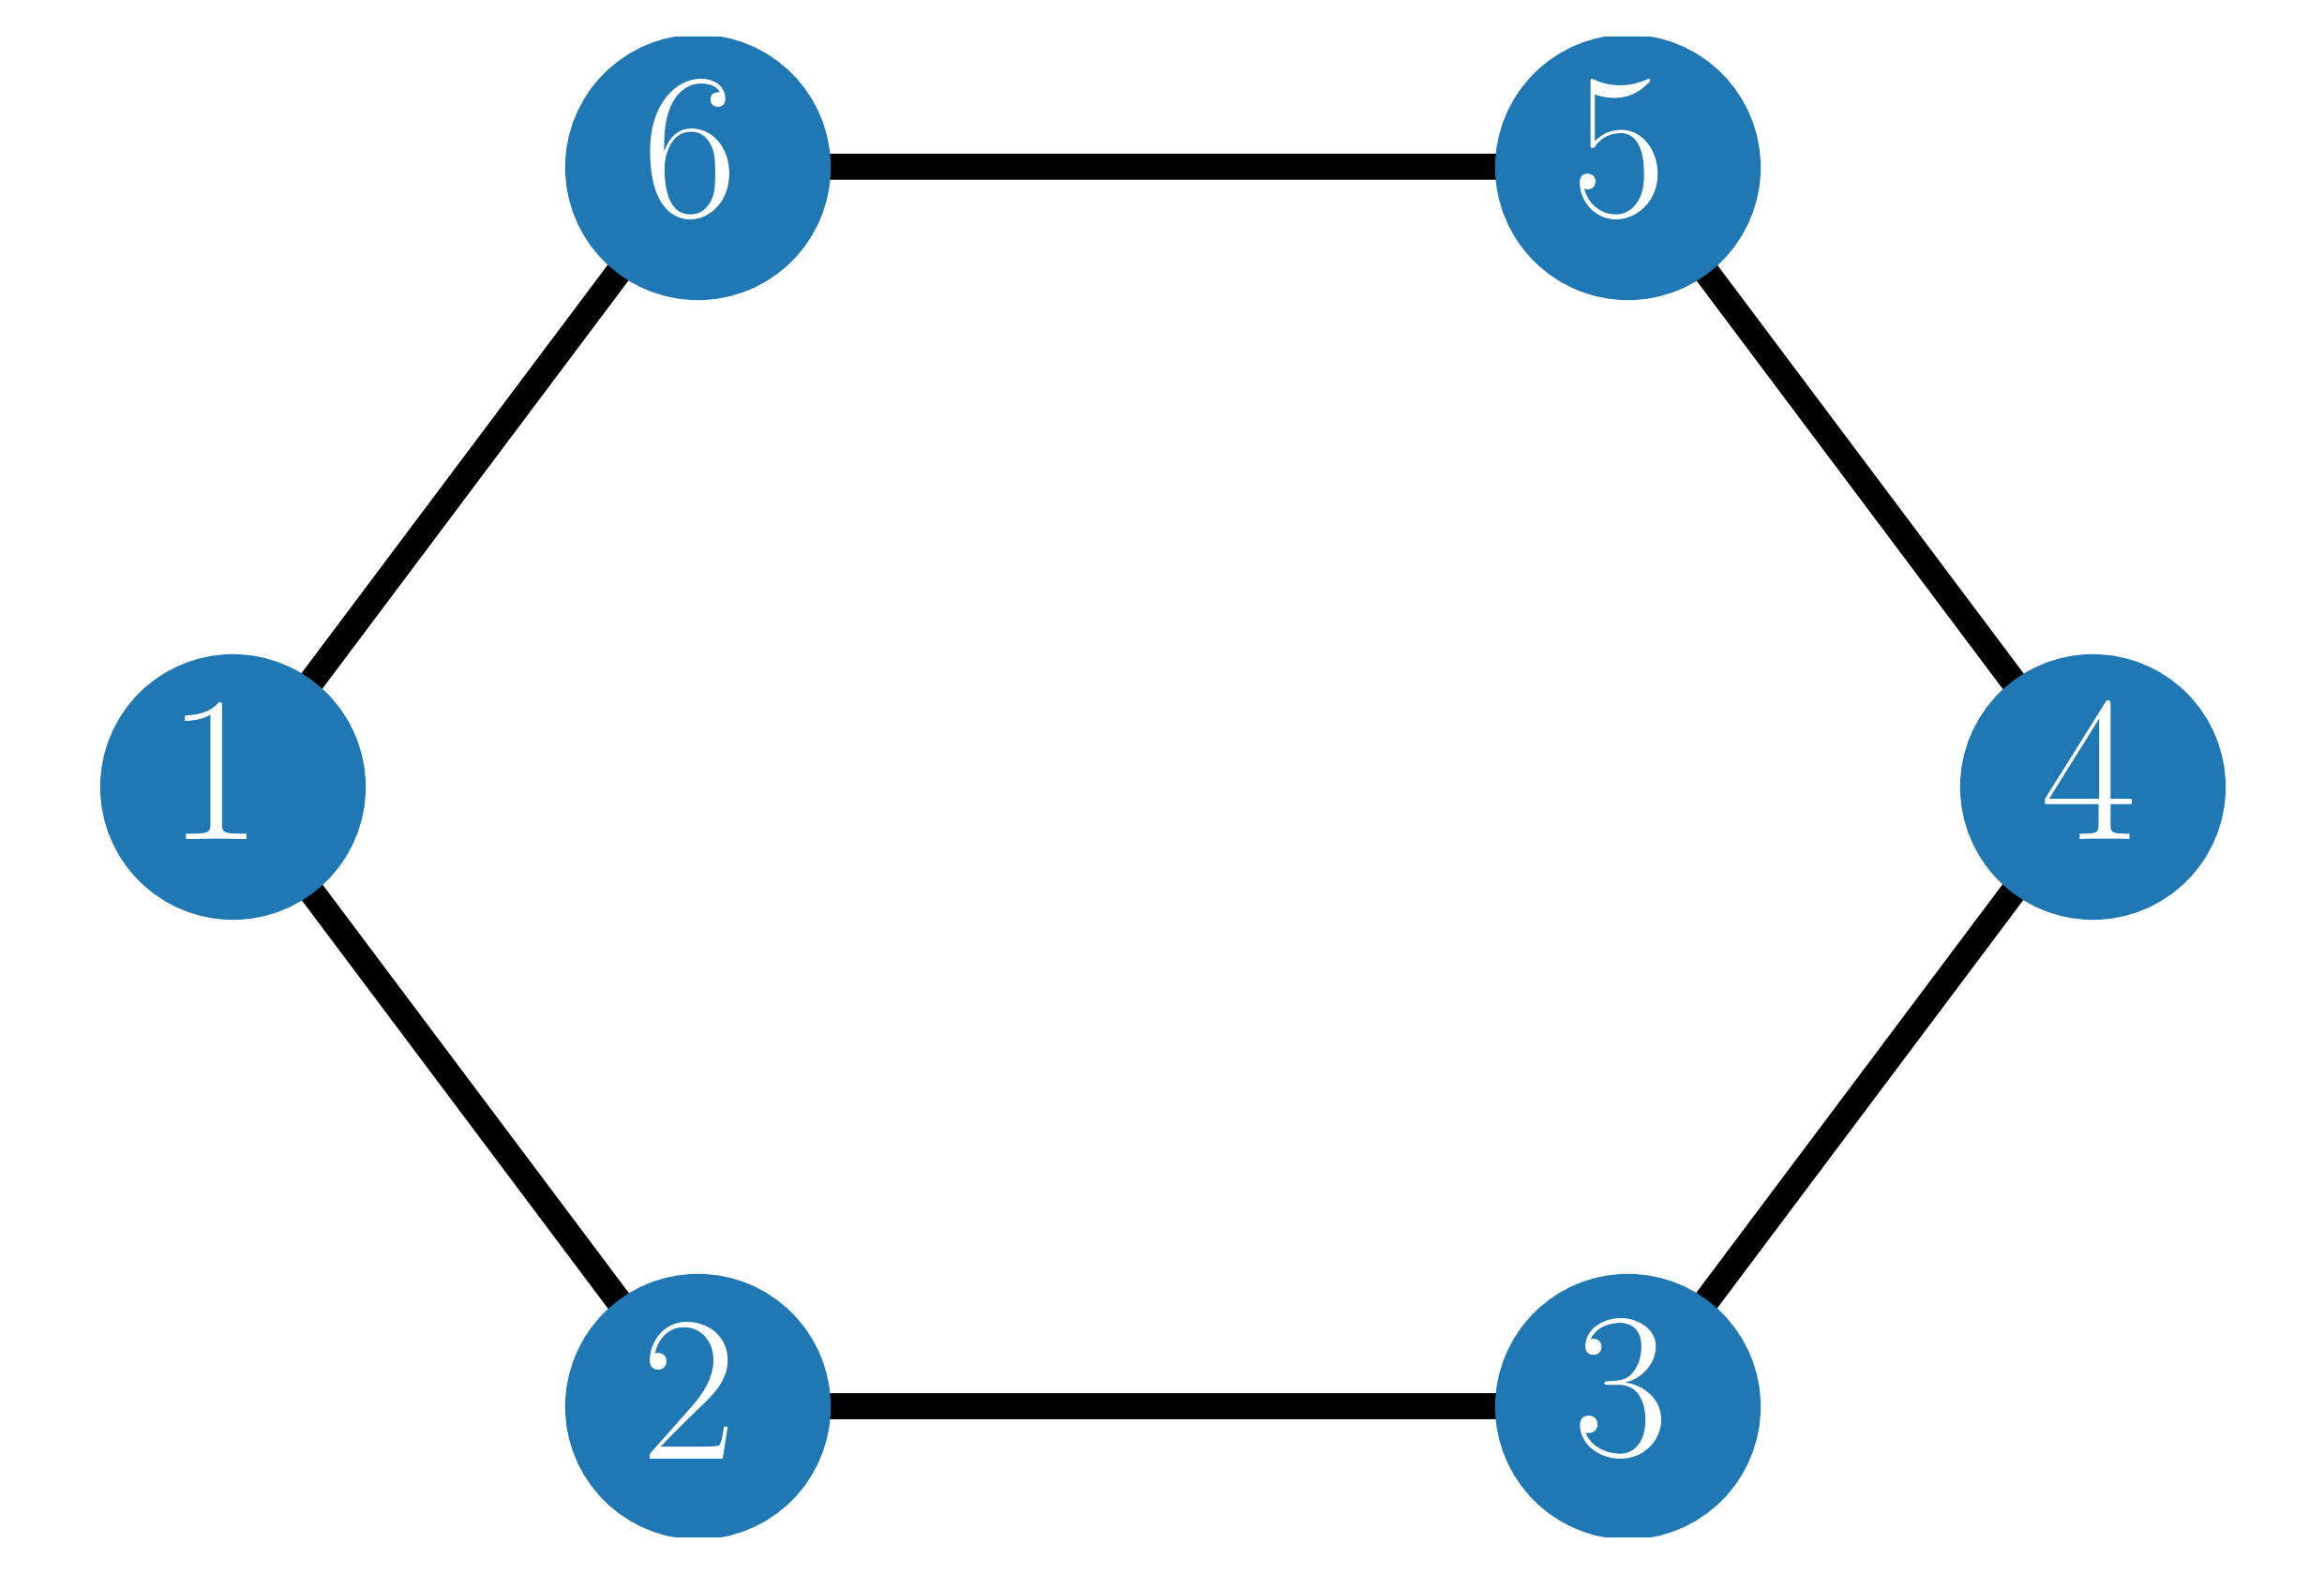
\includegraphics[width=\textwidth]{./figures/shuffled_ring_1.png}
		\caption*{$G_0$}
	\end{subfigure}
	\begin{subfigure}[b]{0.3\textwidth}
		\centering
		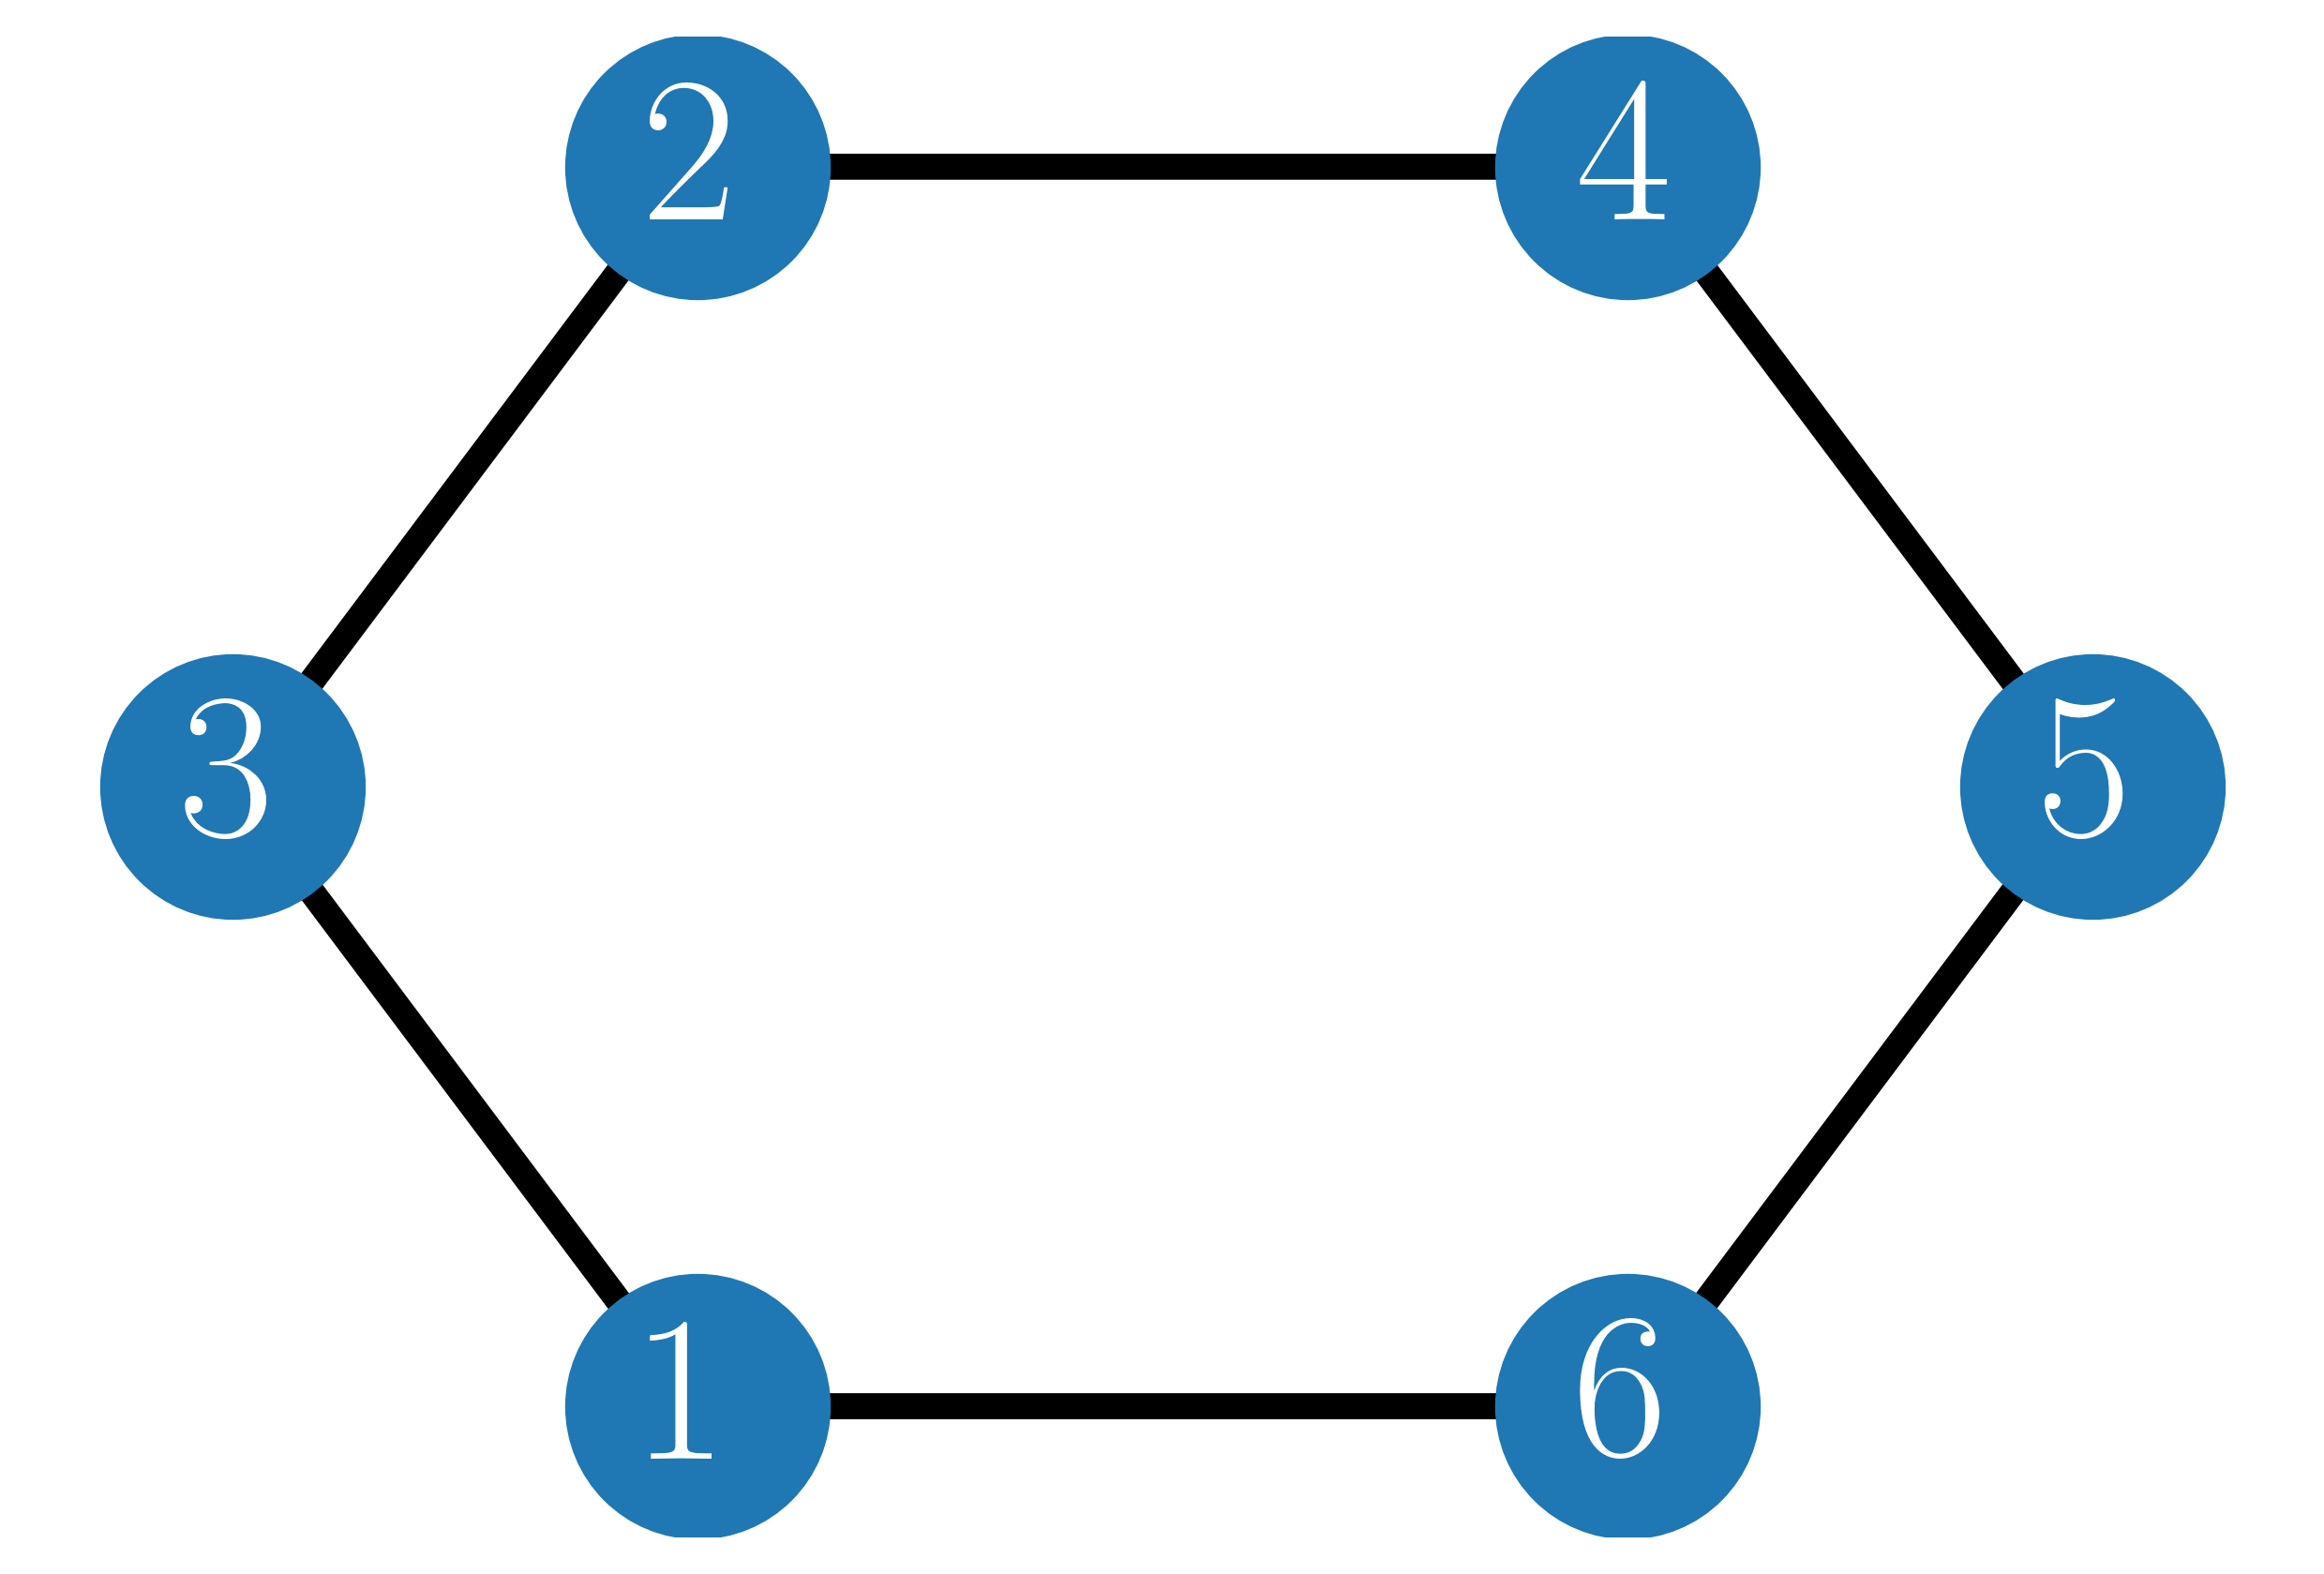
\includegraphics[width=\textwidth]{./figures/shuffled_ring_2.png}
		\caption*{$G_1$}
	\end{subfigure}
	\begin{subfigure}[b]{0.3\textwidth}
		\centering
		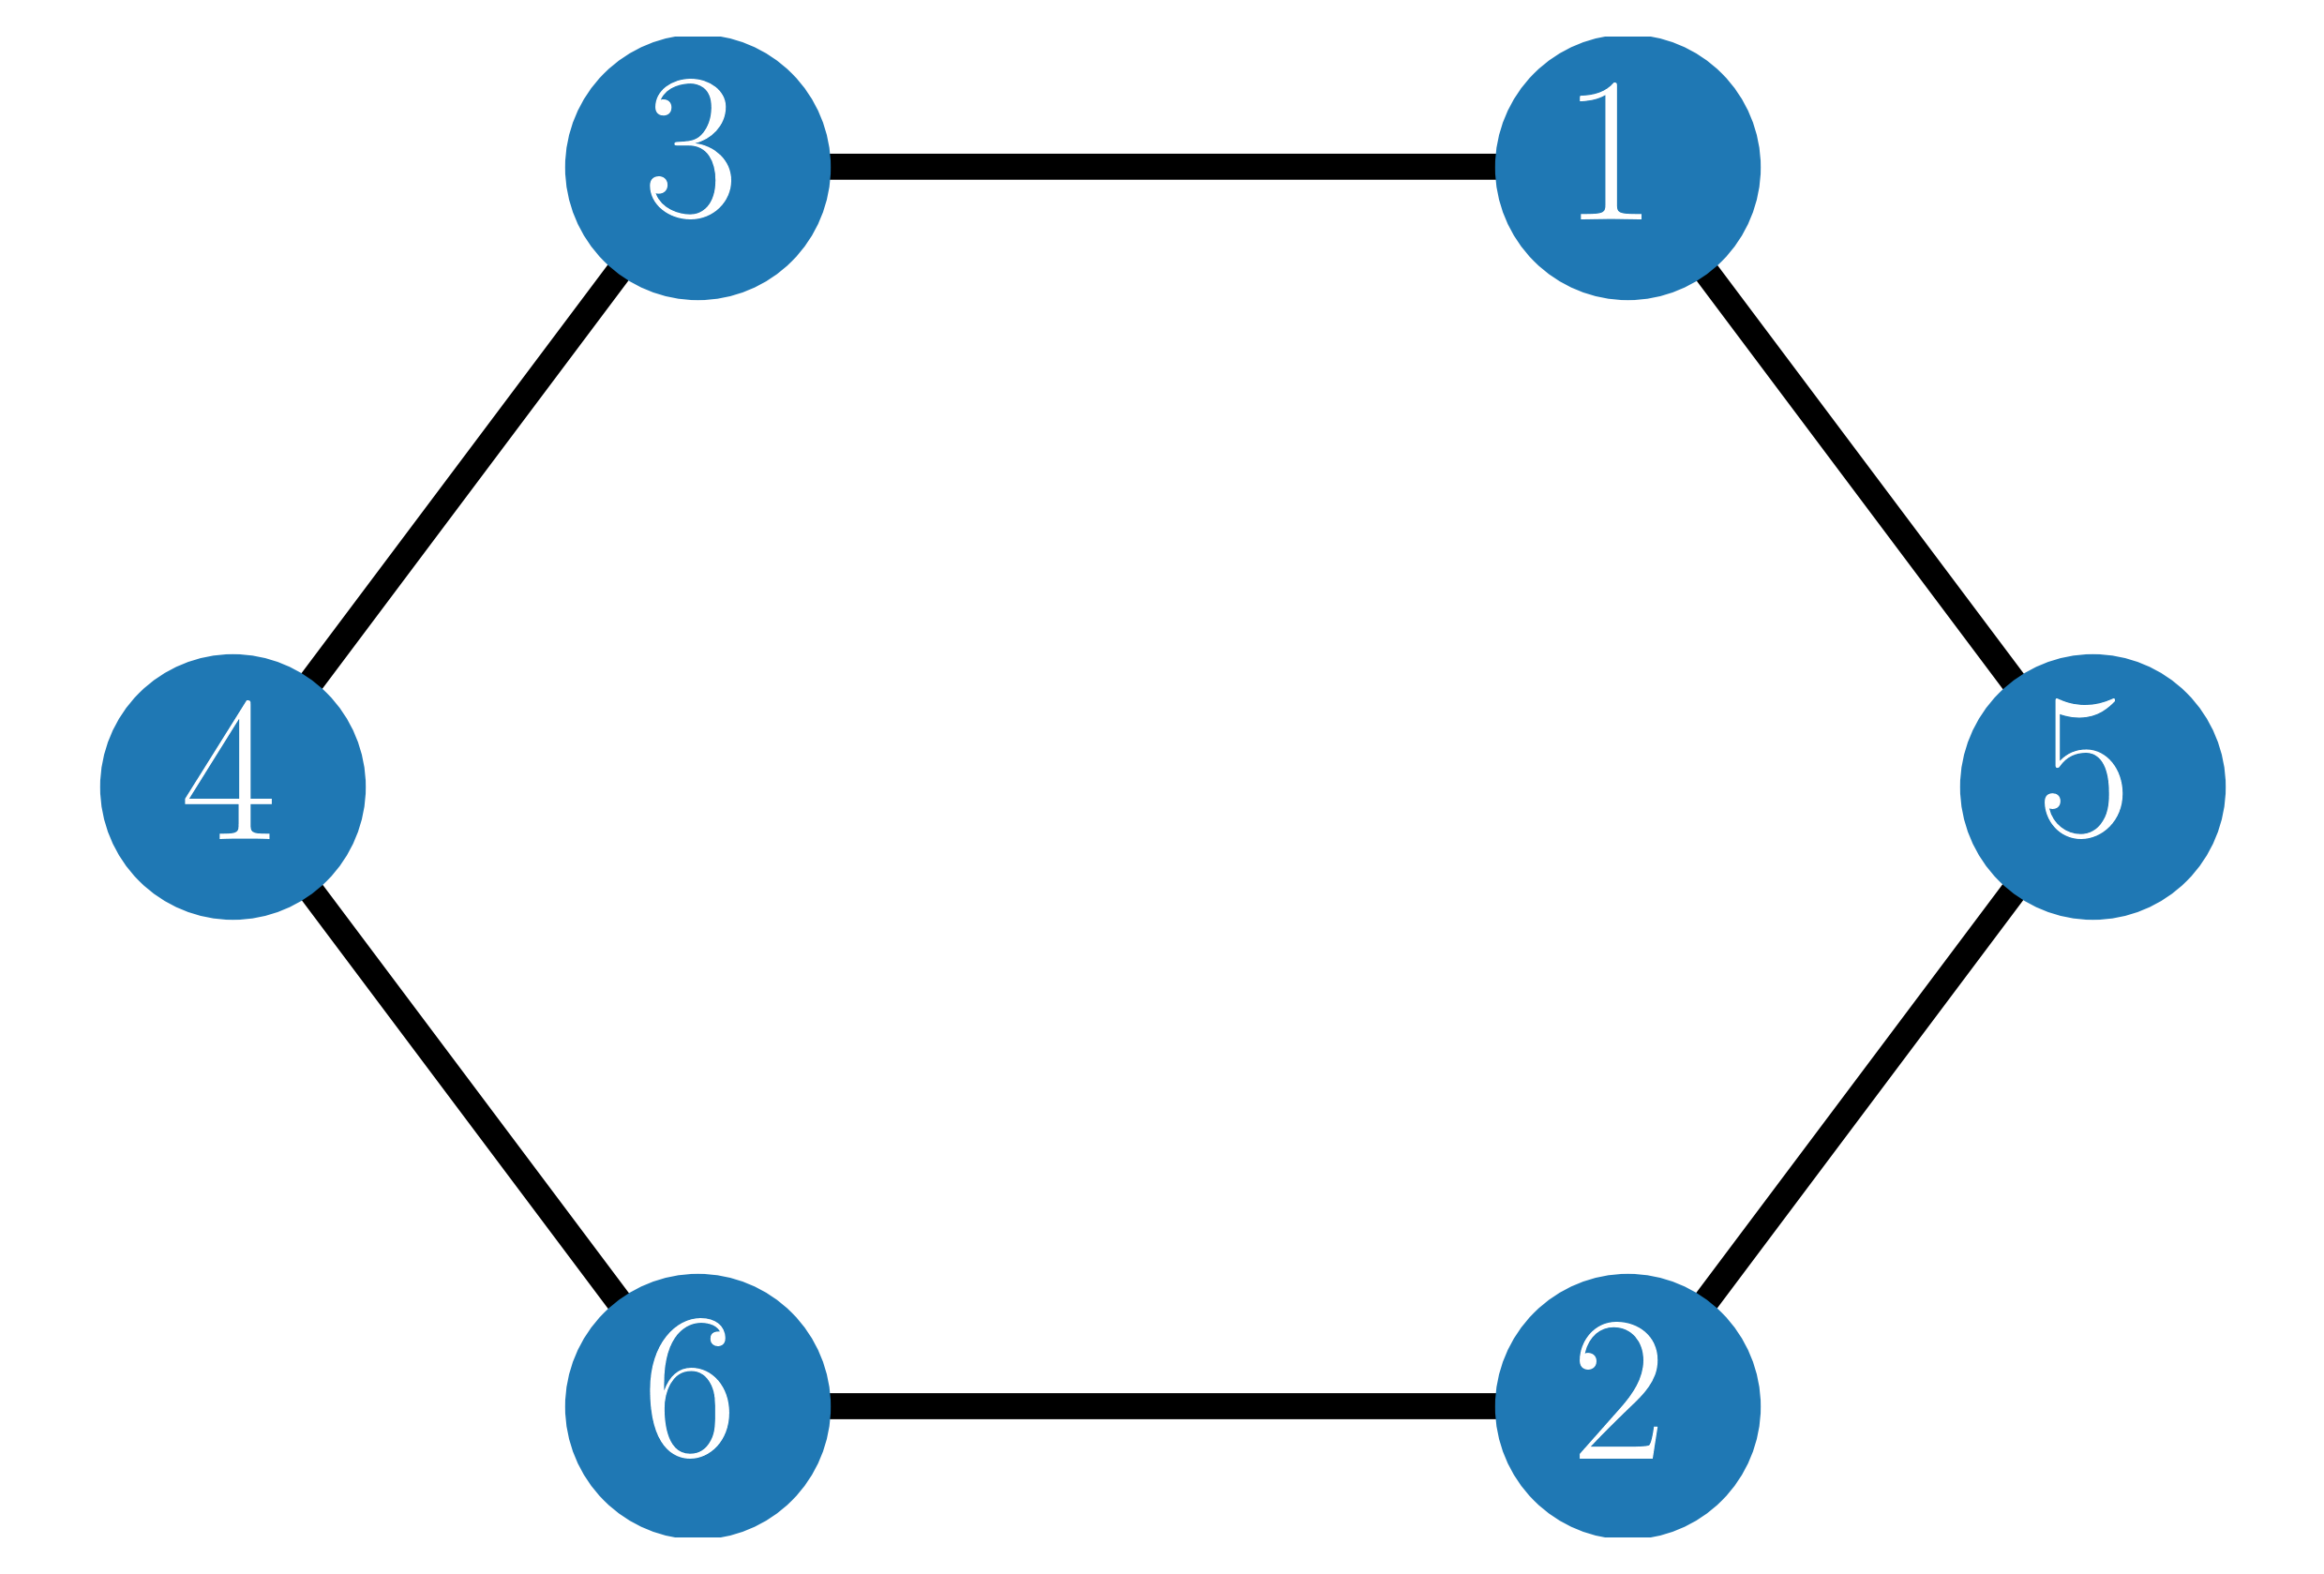
\includegraphics[width=\textwidth]{./figures/shuffled_ring_3.png}
		\caption*{$G_2$}
	\end{subfigure}
	\caption{First three topologies of an example Shuffled Ring Network}
	\label{fig:shuffledRingExample}
\end{figure}

In Figure \ref{fig:shuffledRingExample} we see an example of the first three topologies in a shuffled ring network. Each topology is always a ring, but the order of the nodes is selected uniformly at random each round.

We now use Theorem \ref{theorem:AsyncUpperBound} to bound the spreading time on the Shuffled Ring Network.

\begin{theorem}
	w.h.p the spreading time of Algorithm \ref{NodeCentricAsyncAlgorithm} on the Shuffled Ring Network is at most $\mathcal{O}(n \log n)$.
\end{theorem}

\begin{proof}
	By Theorem \ref{theorem:AsyncUpperBound} we have that w.h.p the rumour spreads in time at most 
	$$
		\min \left\{t : \sum_{k=0}^t \Phi(G_k)\rho(G_k) \geq C \log n \right\} 
	$$
	By computing this quantity explicitly with the conductance and diligence results for the ring graph from Theorem \ref{theorem:ringCompleteAsyncBound} we obtain
	\begin{align*}
		\min \left\{t : \sum_{k=0}^t \Phi(G_k)\rho(G_k) \geq C \log n \right\} 
		&= \min \left\{t : t \Phi(R)\rho(R) \geq C \log n \right\} \\
		&= \min \left\{t : t \Phi(R)\rho(R) \geq C \log n \right\} \\
		&= \ceil*{\frac{C \log n}{\Phi(R)\rho(R)}} \\
		&= \ceil*{\frac{C}{2}n \log n}
	\end{align*}
\end{proof}

We see that the bound we obtain for the spreading time on the Shuffled Ring Network is a factor of $n$ larger than the Ring-Complete Alternating Network, due to the loss of the high-connectivity complete topologies. 

Now we compare the bound we have obtained with simulated spreading times on the Shuffled Ring Network.

\begin{figure}[h]
	\centering
	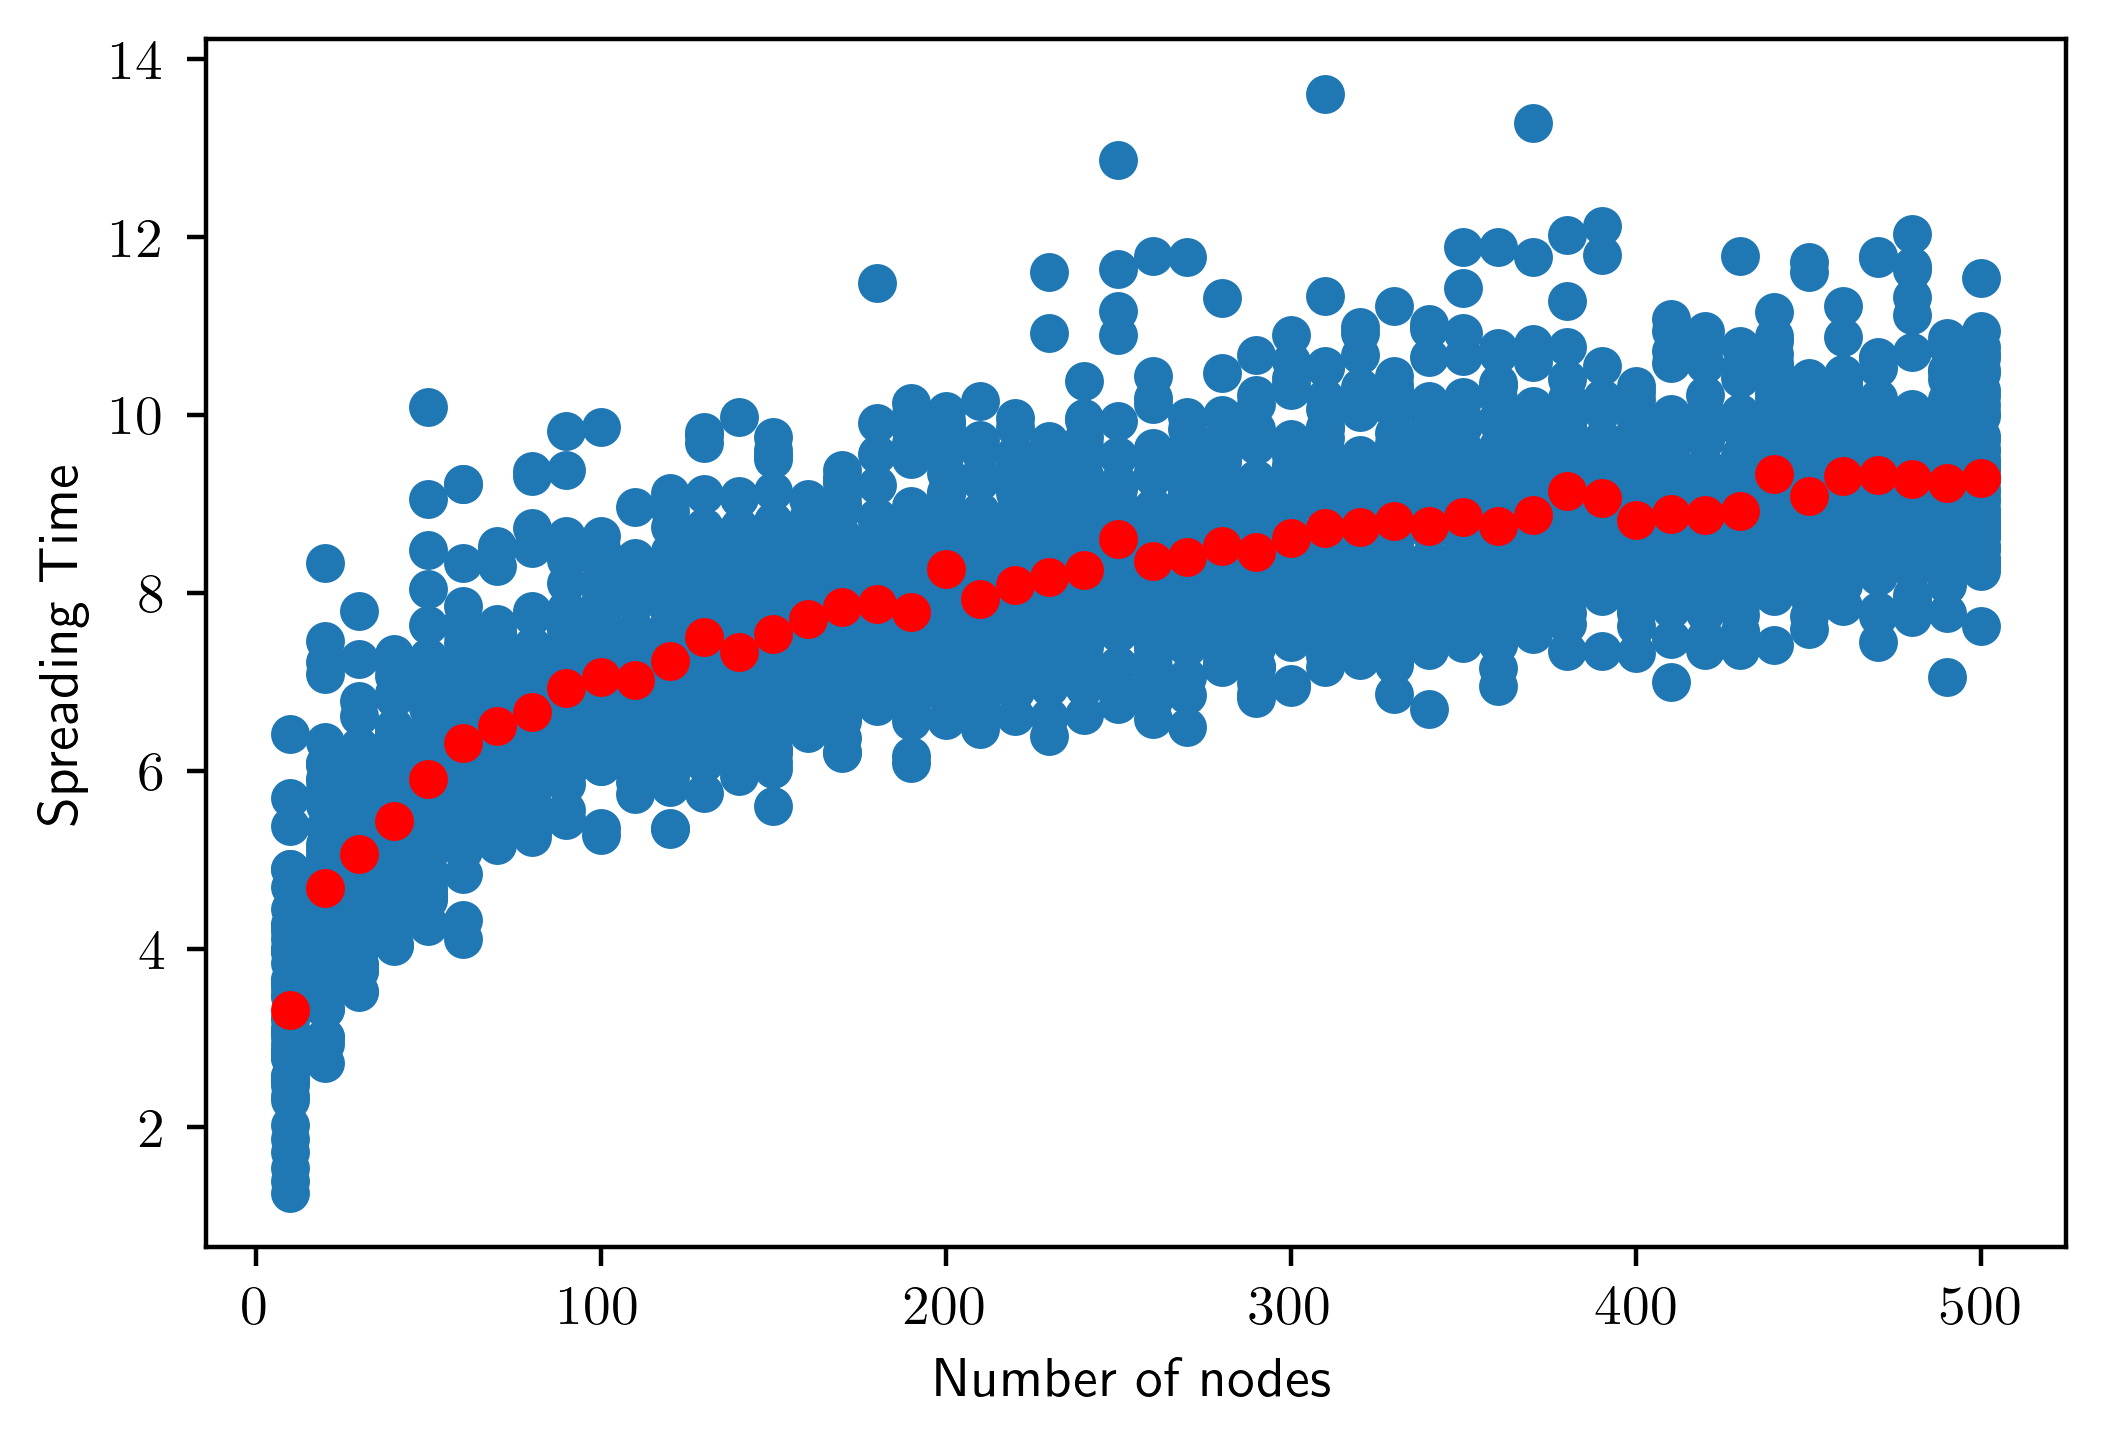
\includegraphics[width=1\textwidth]{./figures/shuffle_ring_simulation_results.png}
	\caption{Results of shuffled ring spreading time simulations}
	\label{fig:shuffleRingSimResults}
\end{figure}

In Figure \ref{fig:shuffledRingExample} we have used the same methods of analysis as in Figure \ref{fig:alternatingSimResults}. However, for this network, the spreading times grow like $\mathcal{O}(\log n)$, which is slower than in $\mathcal{A}$.
The $\mathcal{O}(n \log n)$ bound given by Theorem $\ref{theorem:AsyncUpperBound}$ is larger than the true spreading times by a factor of $\mathcal{O}(n)$ in asymptotic scaling. Hence, the bound is very weak, and is unlikely to be useful in practice. But why is it the case that the bound is so weak for $\mathcal{S}$?

To answer this question, we investigate the spreading time on the static ring graph.

\subsection{Static Ring}

\begin{definition}
	Static Ring Network $\mathcal{R}$

	\noindent
	Let $R$ be a cycle graph on $n$ nodes. The Static Ring Network is the network consisting of the same ring $R$ for every topology, i.e. $\mathcal{R} = (G_t)_{t \in \mathbb{N}}$ where $G_t = R$ for all $t \in \mathbb{N}$. 
\end{definition}

\begin{theorem}\label{theorem:staticRingAsyncBound}
	w.h.p the spreading time of Algorithm \ref{NodeCentricAsyncAlgorithm} on the Static Ring Network is at most $\mathcal{O}(n \log n)$.
\end{theorem}

\begin{proof}
	We notice that the Shuffled Ring Network and Static Ring Network networks are isomorphic. Since the connectivity metrics are invariant to node renaming, both networks have the same conductance and diligence in each round. Since Theorem \ref{theorem:AsyncUpperBound} is only dependent on the sequence of connectivity metrics, we obtain the same bound for the Static Ring Network and the Shuffled Ring Network.
\end{proof} 

Now we investigate the simulated spreading times on the Static Ring Graph.

\begin{figure}[h]
	\centering
	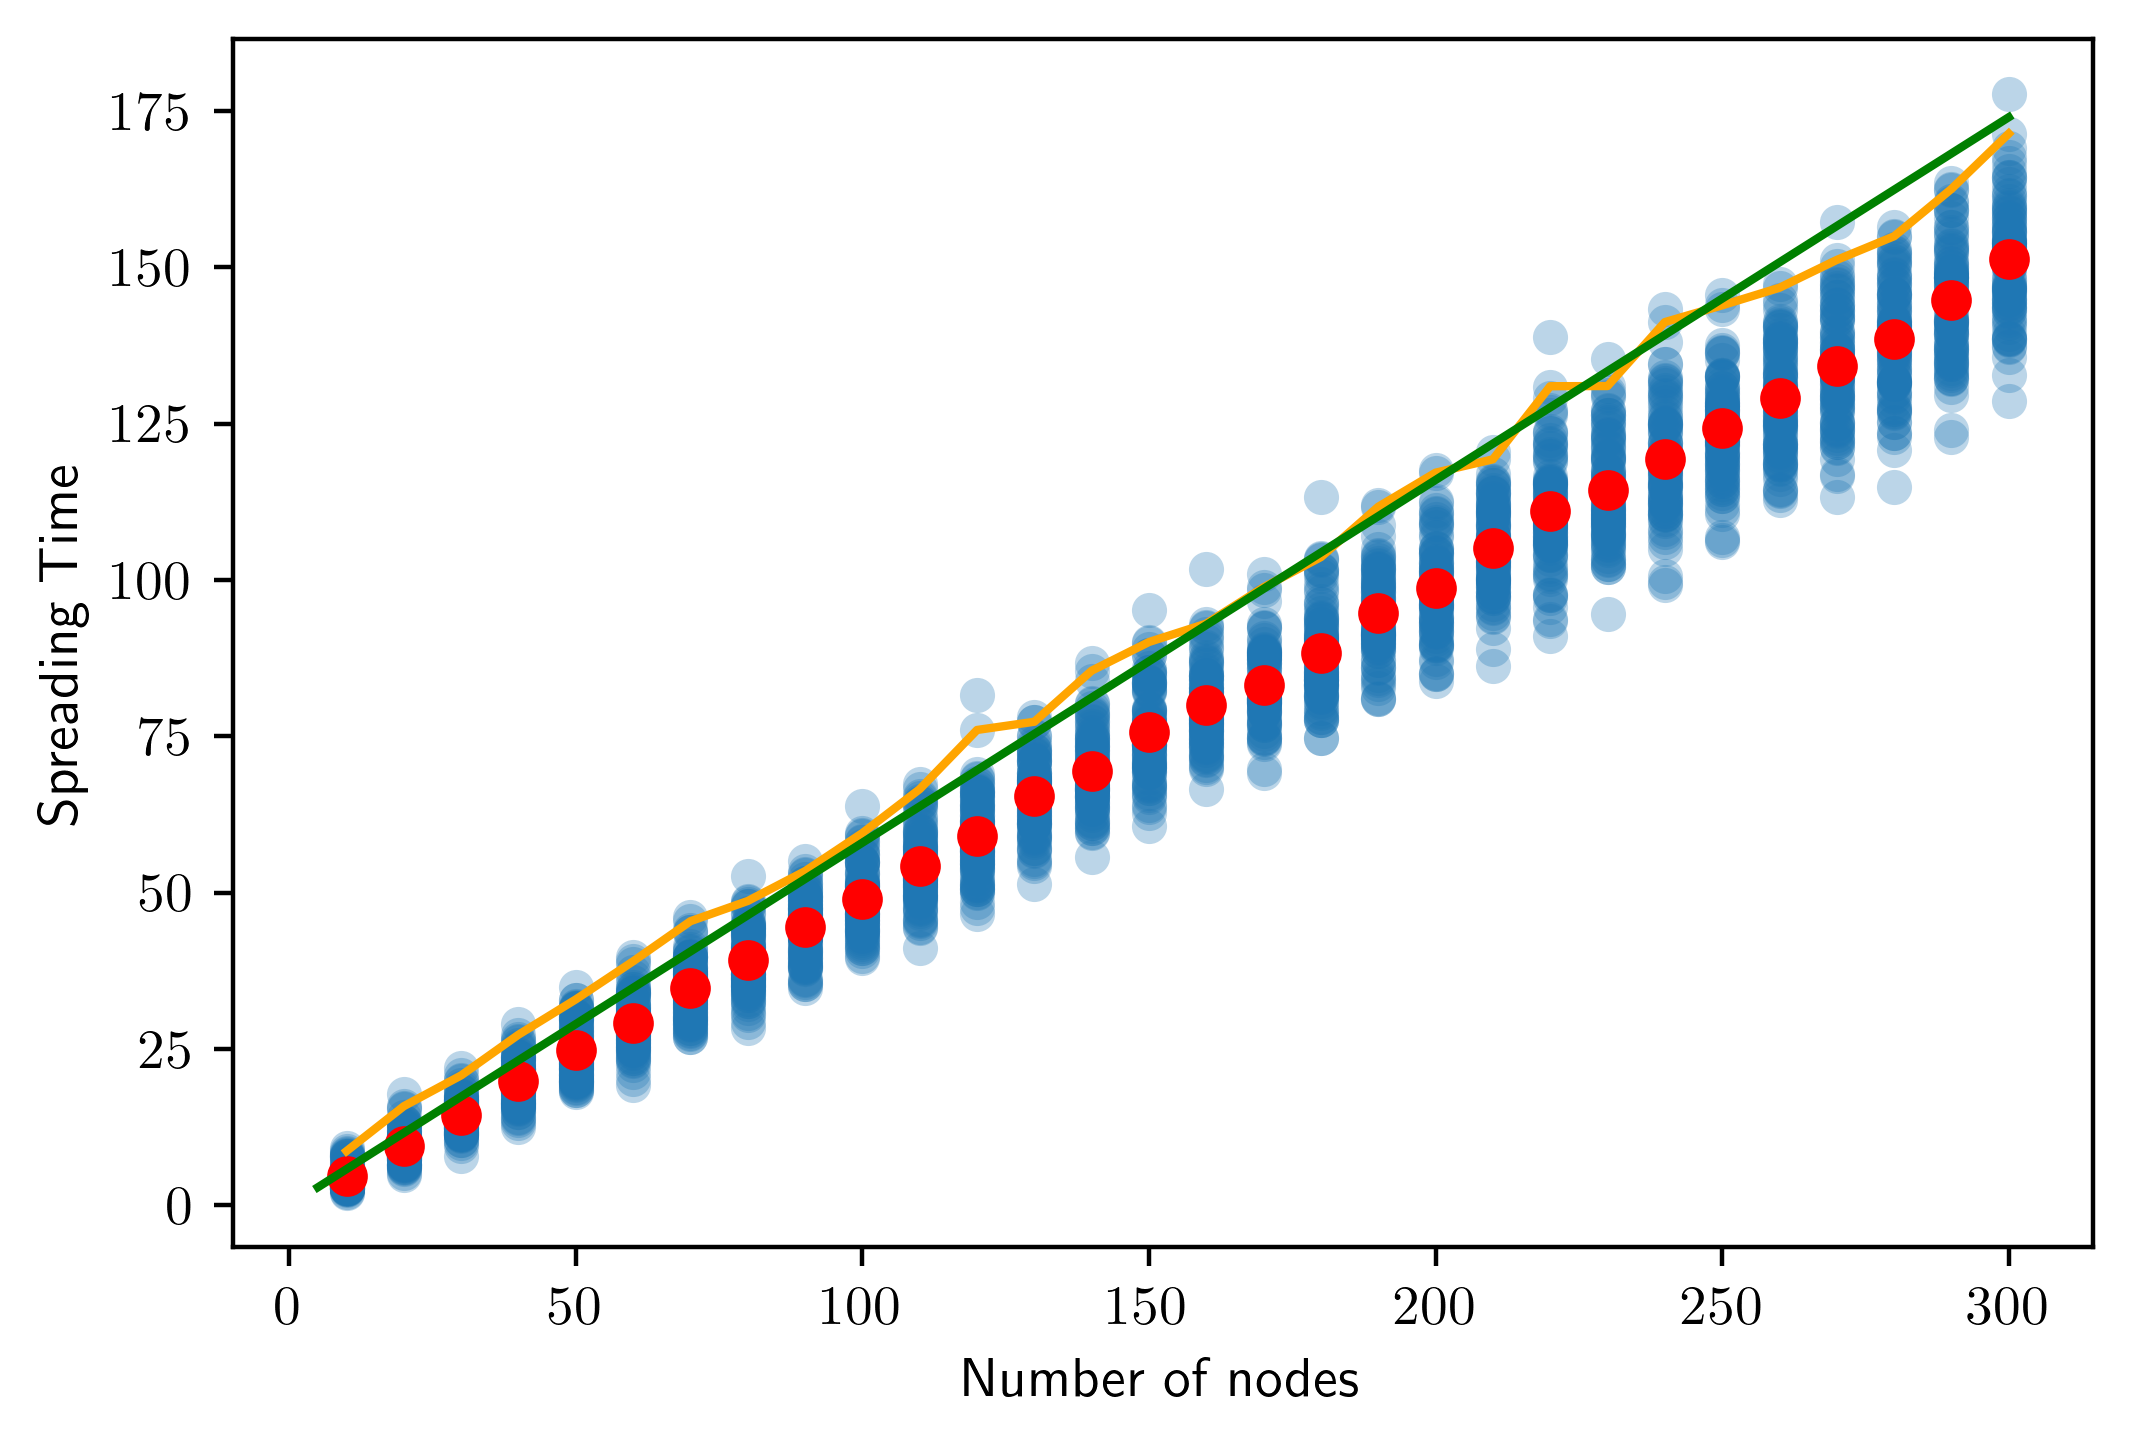
\includegraphics[width=1\textwidth]{./figures/static_ring_simulation_results.png}
	\caption{Results of static ring spreading time simulations}
	\label{fig:staticRingSimResults}
\end{figure}

We see from the simulations on the Static Ring network that the spreading time grows linearly with the number of nodes in the network. Notice that this is significantly slower than the logarithmic growth seen in the Shuffled Ring simulations, despite the fact that the networks are isomorphic.
Since the true spreading time growth for Static Ring network is linear, the $\mathcal{O}(n \log n)$ bound given by Theorem \ref{theorem:AsyncUpperBound} is much tighter for this network, and is only a factor of $\mathcal{O}(\log n)$ larger than the simulated spreading times.

We investigate why the rumour spreads faster on the Shuffled Ring Network by comparing how the rumour spreads in the Shuffled Ring and Static Ring networks.

By the superposition and thinning properties of the Poisson process, we can interpret the operation of Algorithm \ref{NodeCentricAsyncAlgorithm} as picking a node at random according to the arrival times of rate $n$ Poisson process,
before picking a random neighbour to exchange the rumour with. If one of the nodes is aware of the rumour and the other is not, a spreading event will occur.
In the ring topology all nodes have the same degree, so we can further simplify the interpretation of the spreading process as choosing a present edge uniformly at random according to the arrival times of a rate $n$ Poisson process. Thus, the greater the proportion of active edges to inactive edges, the greater the probability that the chosen edge is active, and triggers a spreading event. More frequent spreading events in turn yield lower spreading times. 

\begin{figure}[h]
	\centering
	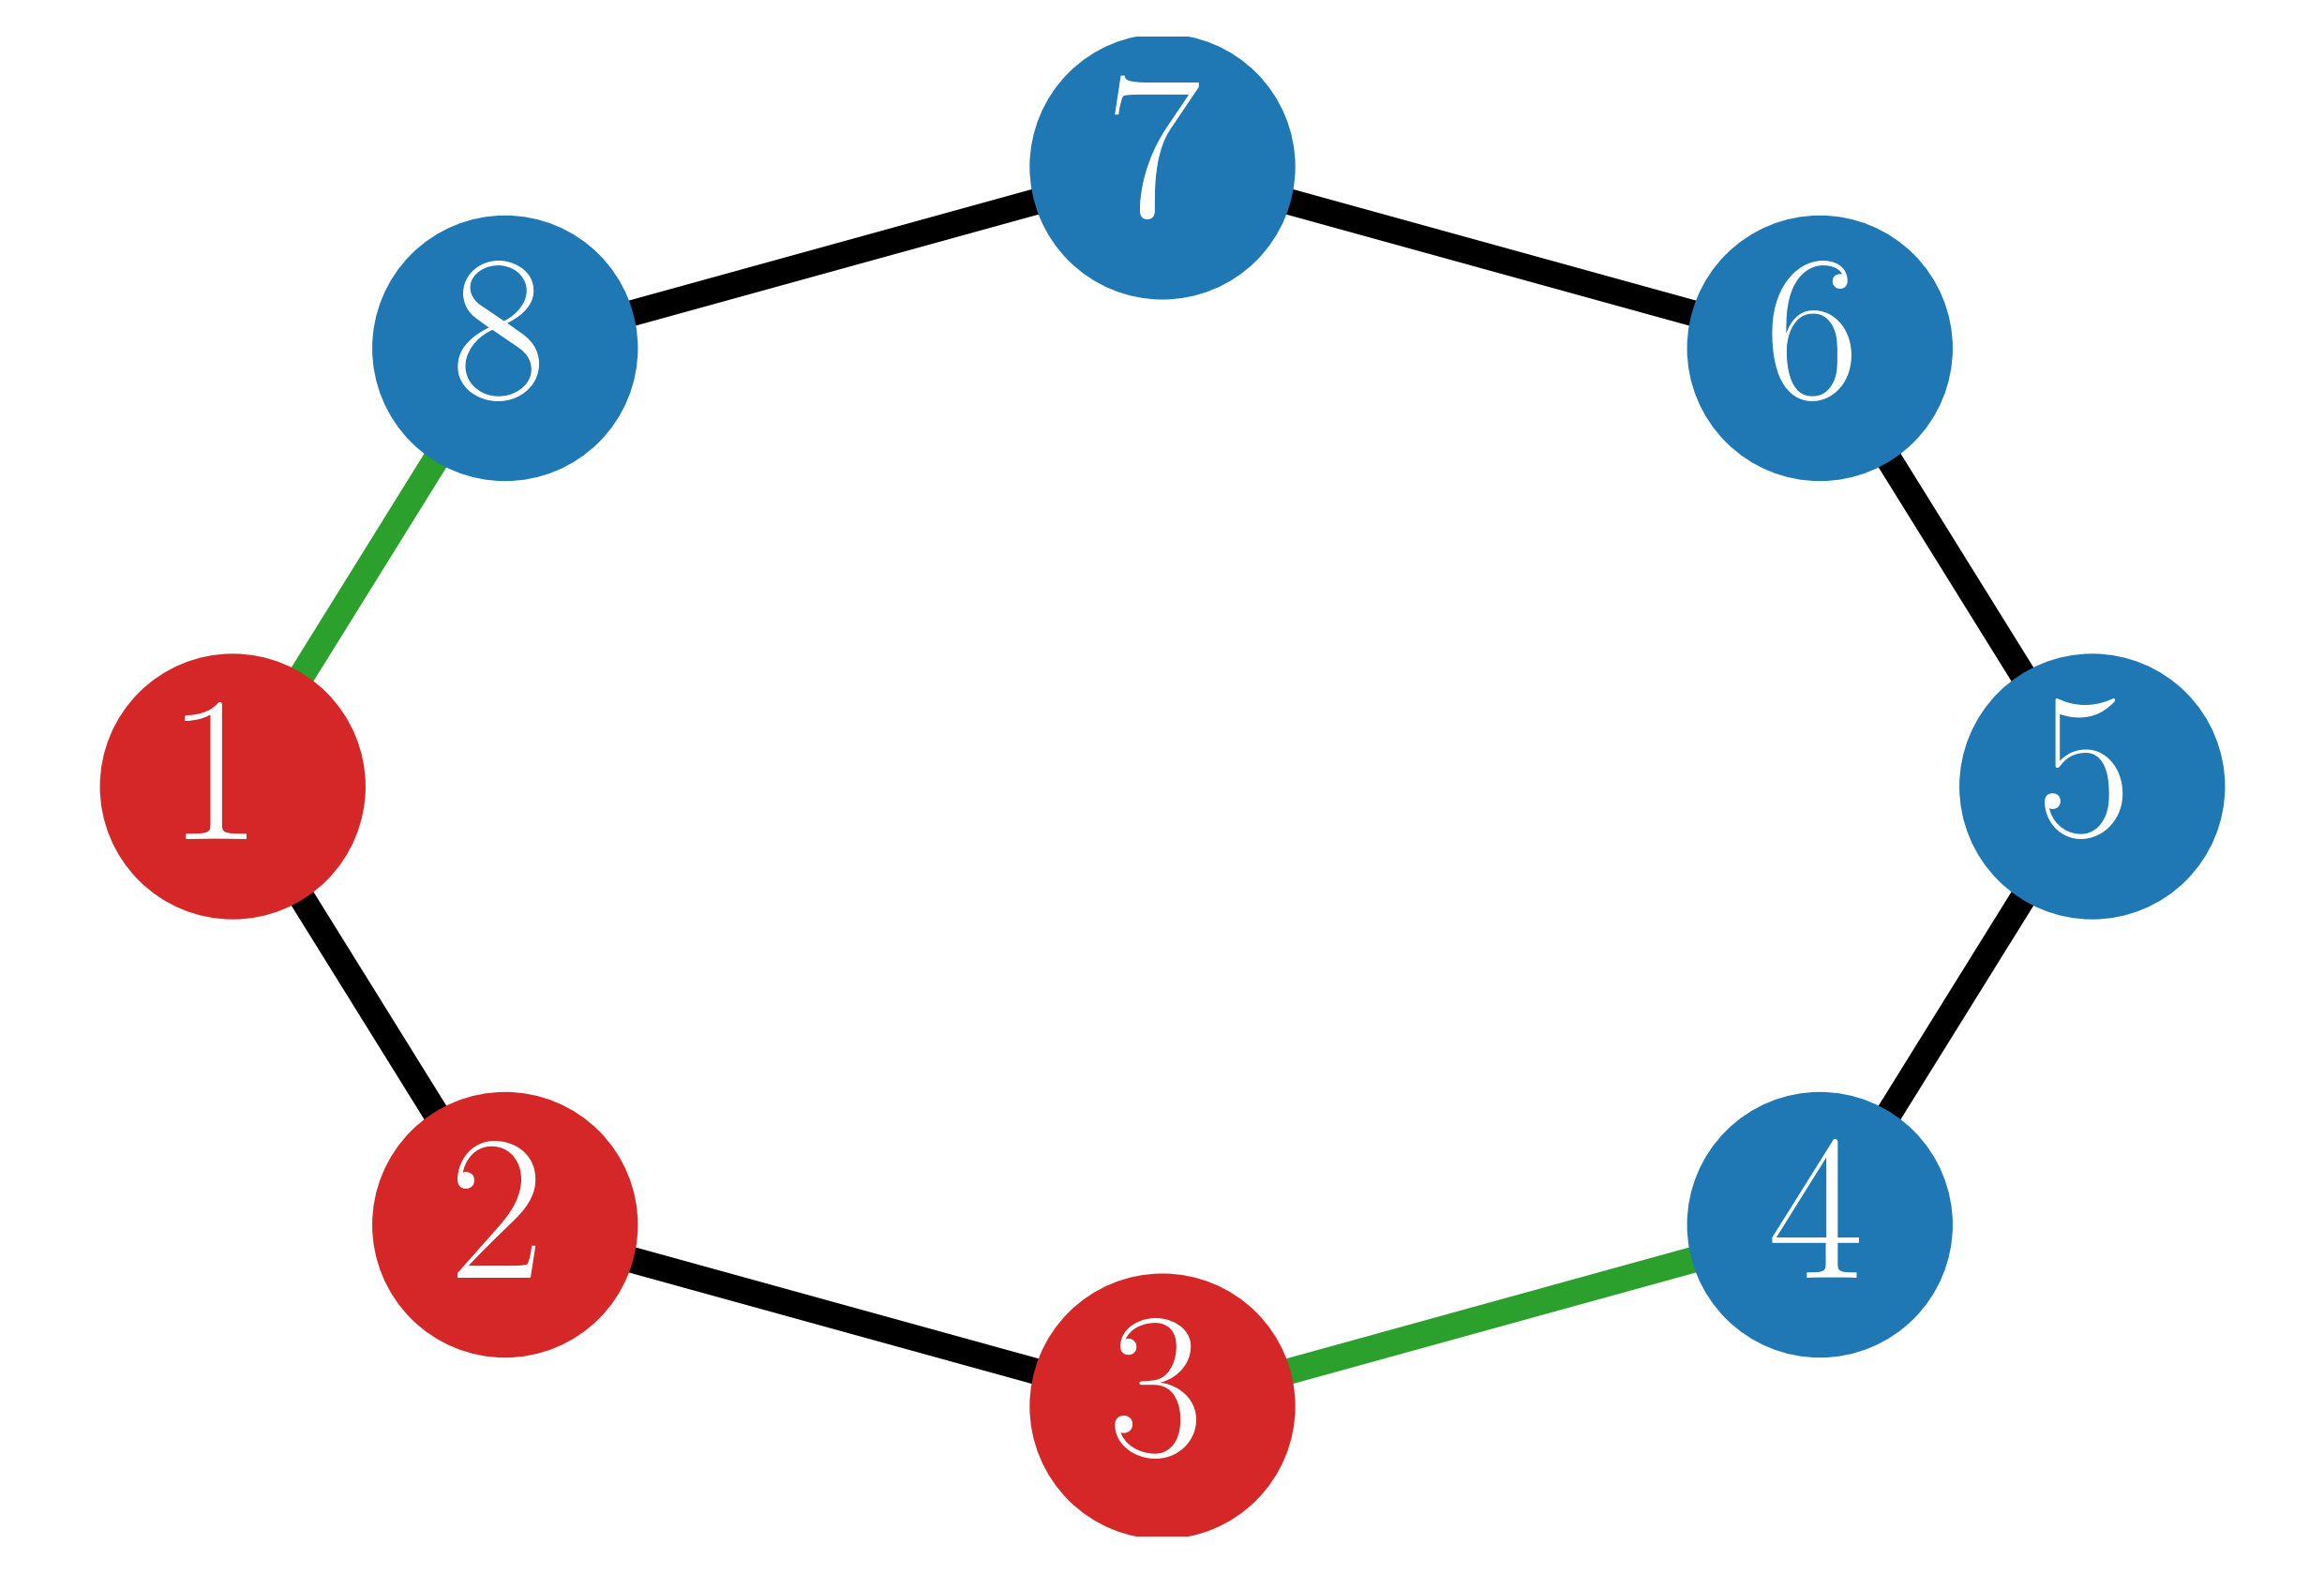
\includegraphics[width=0.49\textwidth]{./figures/static_ring_example_spread.png}
	\caption{Example rumour spread on the Static Ring Network}
	\label{fig:staticRingExampleSpread}
\end{figure}

In the Static Ring Network, we find that at all times there are only two active edges, namely the two edges connecting the contiguous set of informed nodes to the uninformed nodes.  This is illustrated in Figure \ref{fig:staticRingExampleSpread}, where red nodes are aware of the rumour, blue nodes are not aware of the rumour, and green edges highlight active connections along which the rumour could spread.

\begin{figure}[h]
	\centering
    \begin{subfigure}[b]{0.49\textwidth}
		\centering
		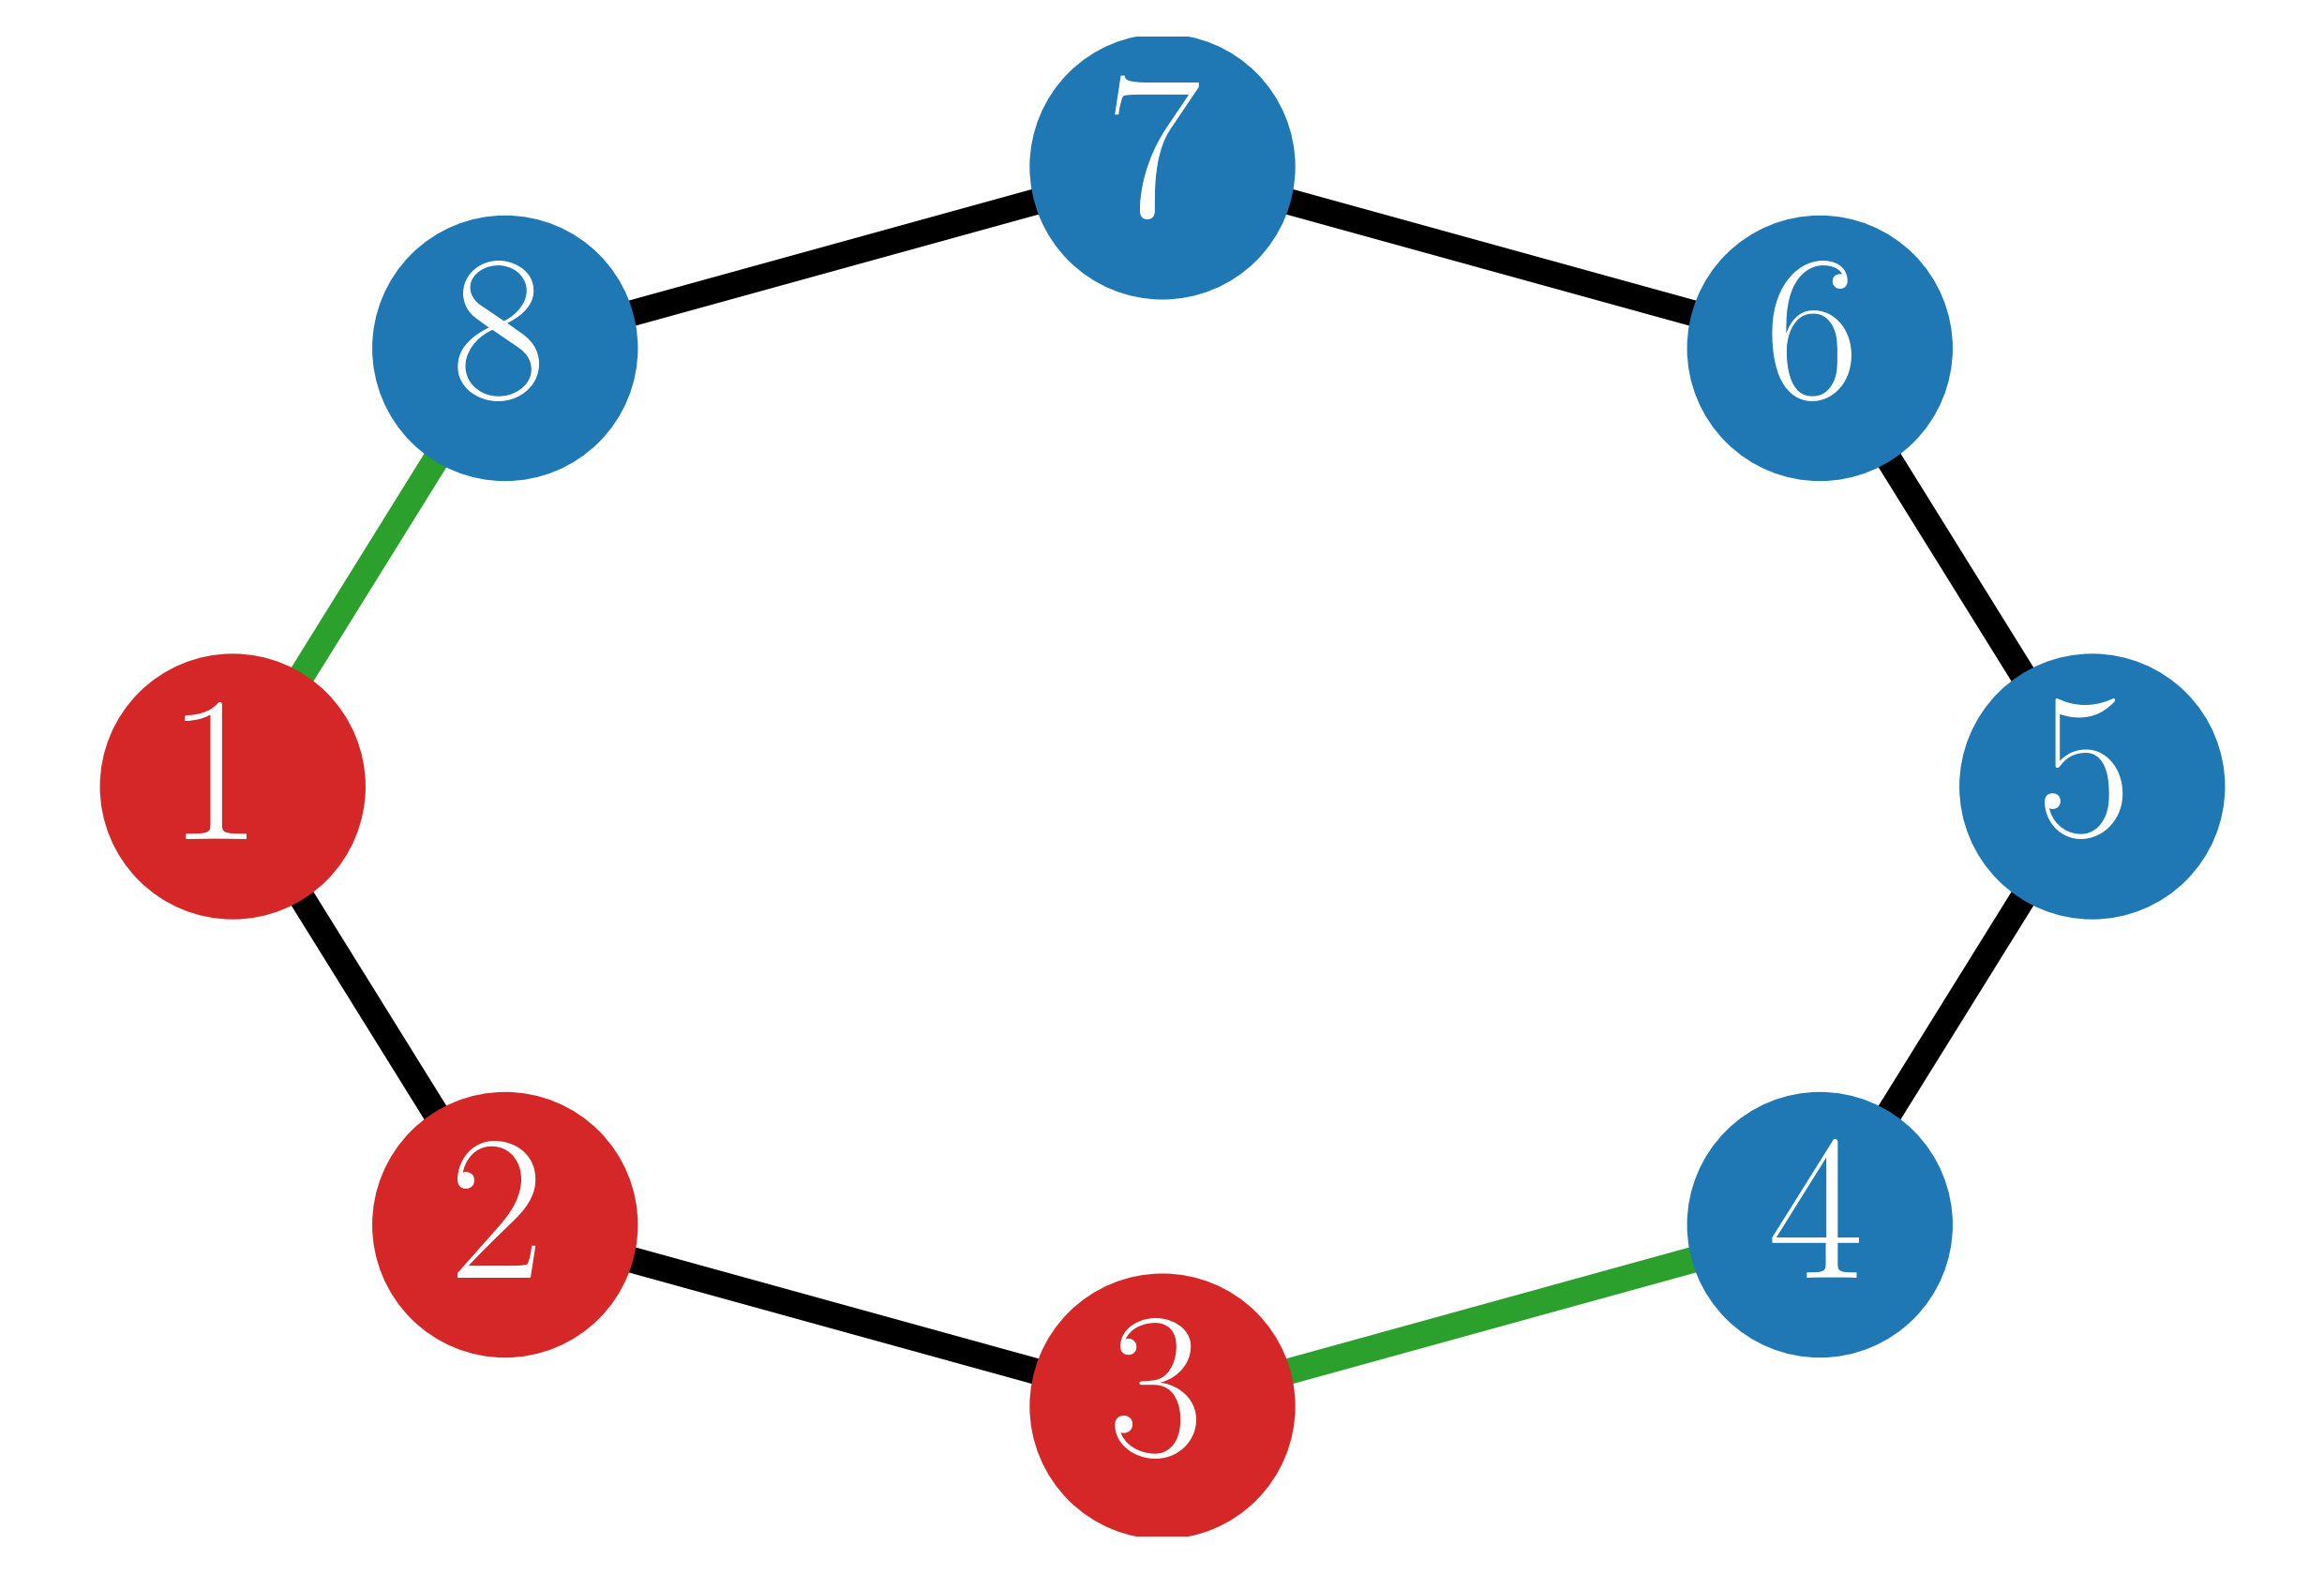
\includegraphics[width=\textwidth]{./figures/static_ring_example_spread.png}
		\caption*{$t=1 - \epsilon$, for all small $\epsilon > 0$}
	\end{subfigure}
	\begin{subfigure}[b]{0.49\textwidth}
		\centering
		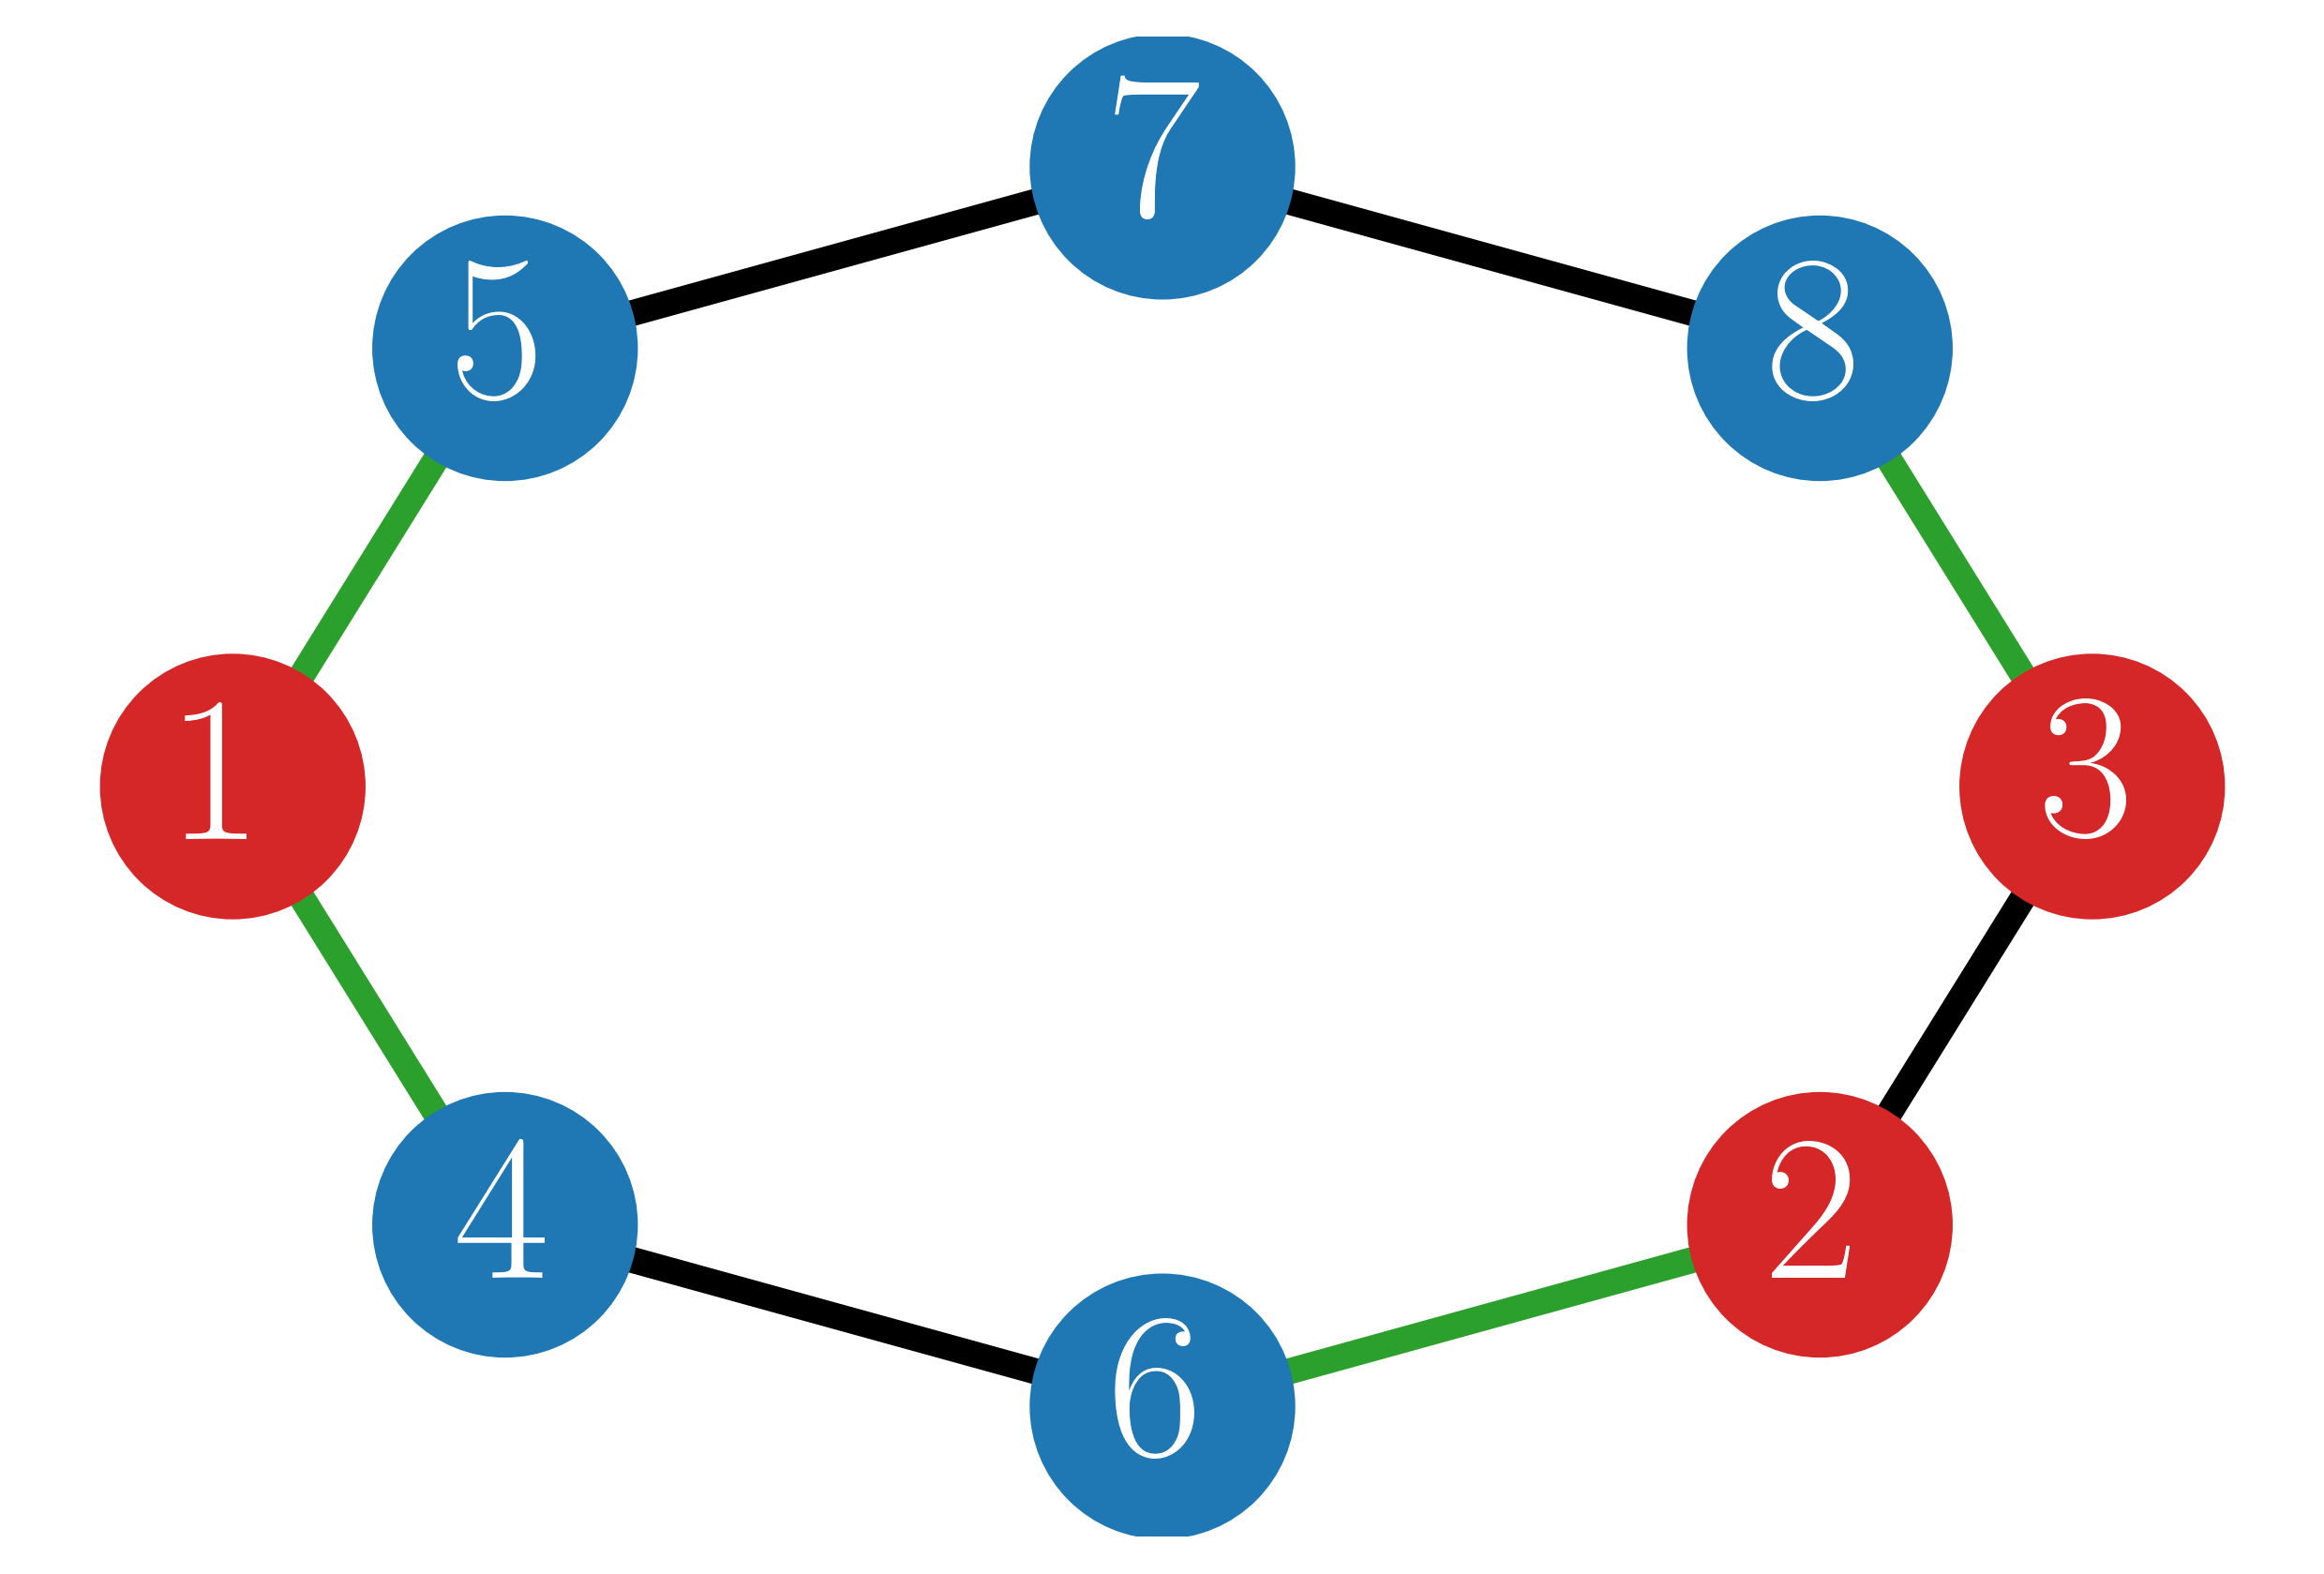
\includegraphics[width=\textwidth]{./figures/shuffled_ring_example_spread.png}
		\caption*{$t=1$}
	\end{subfigure}
	\caption{Example rumour spread on the Shuffled Ring Network}
	\label{fig:shuffledRingExampleSpread}
\end{figure}

Within a round, in the Shuffled Ring Network, the rumour spreads similarly to the Static Network, i.e. by extending the contiguous set of informed nodes. We see this behaviour in the $t = 1 - \epsilon$ case of Figure \ref{fig:shuffledRingExampleSpread}. However, when the network is shuffled at the start of the new round, it is likely that the continuous set of informed nodes is broken up and scattered around the ring, forming multiple continuous sets of informed nodes as seen in the $t=1$ case of Figure \ref{fig:shuffledRingExampleSpread}. Each of these new sets of adjacent informed nodes contributes an additional two active edges.

Hence, the spreading time is longer for the Static Ring Network, as the Static Ring Network is limited to 2 active edges at any time, whereas the Shuffled Ring Network could have many more. We observe the effects of this behaviour in simulations.

\begin{figure}[h]
	\centering
	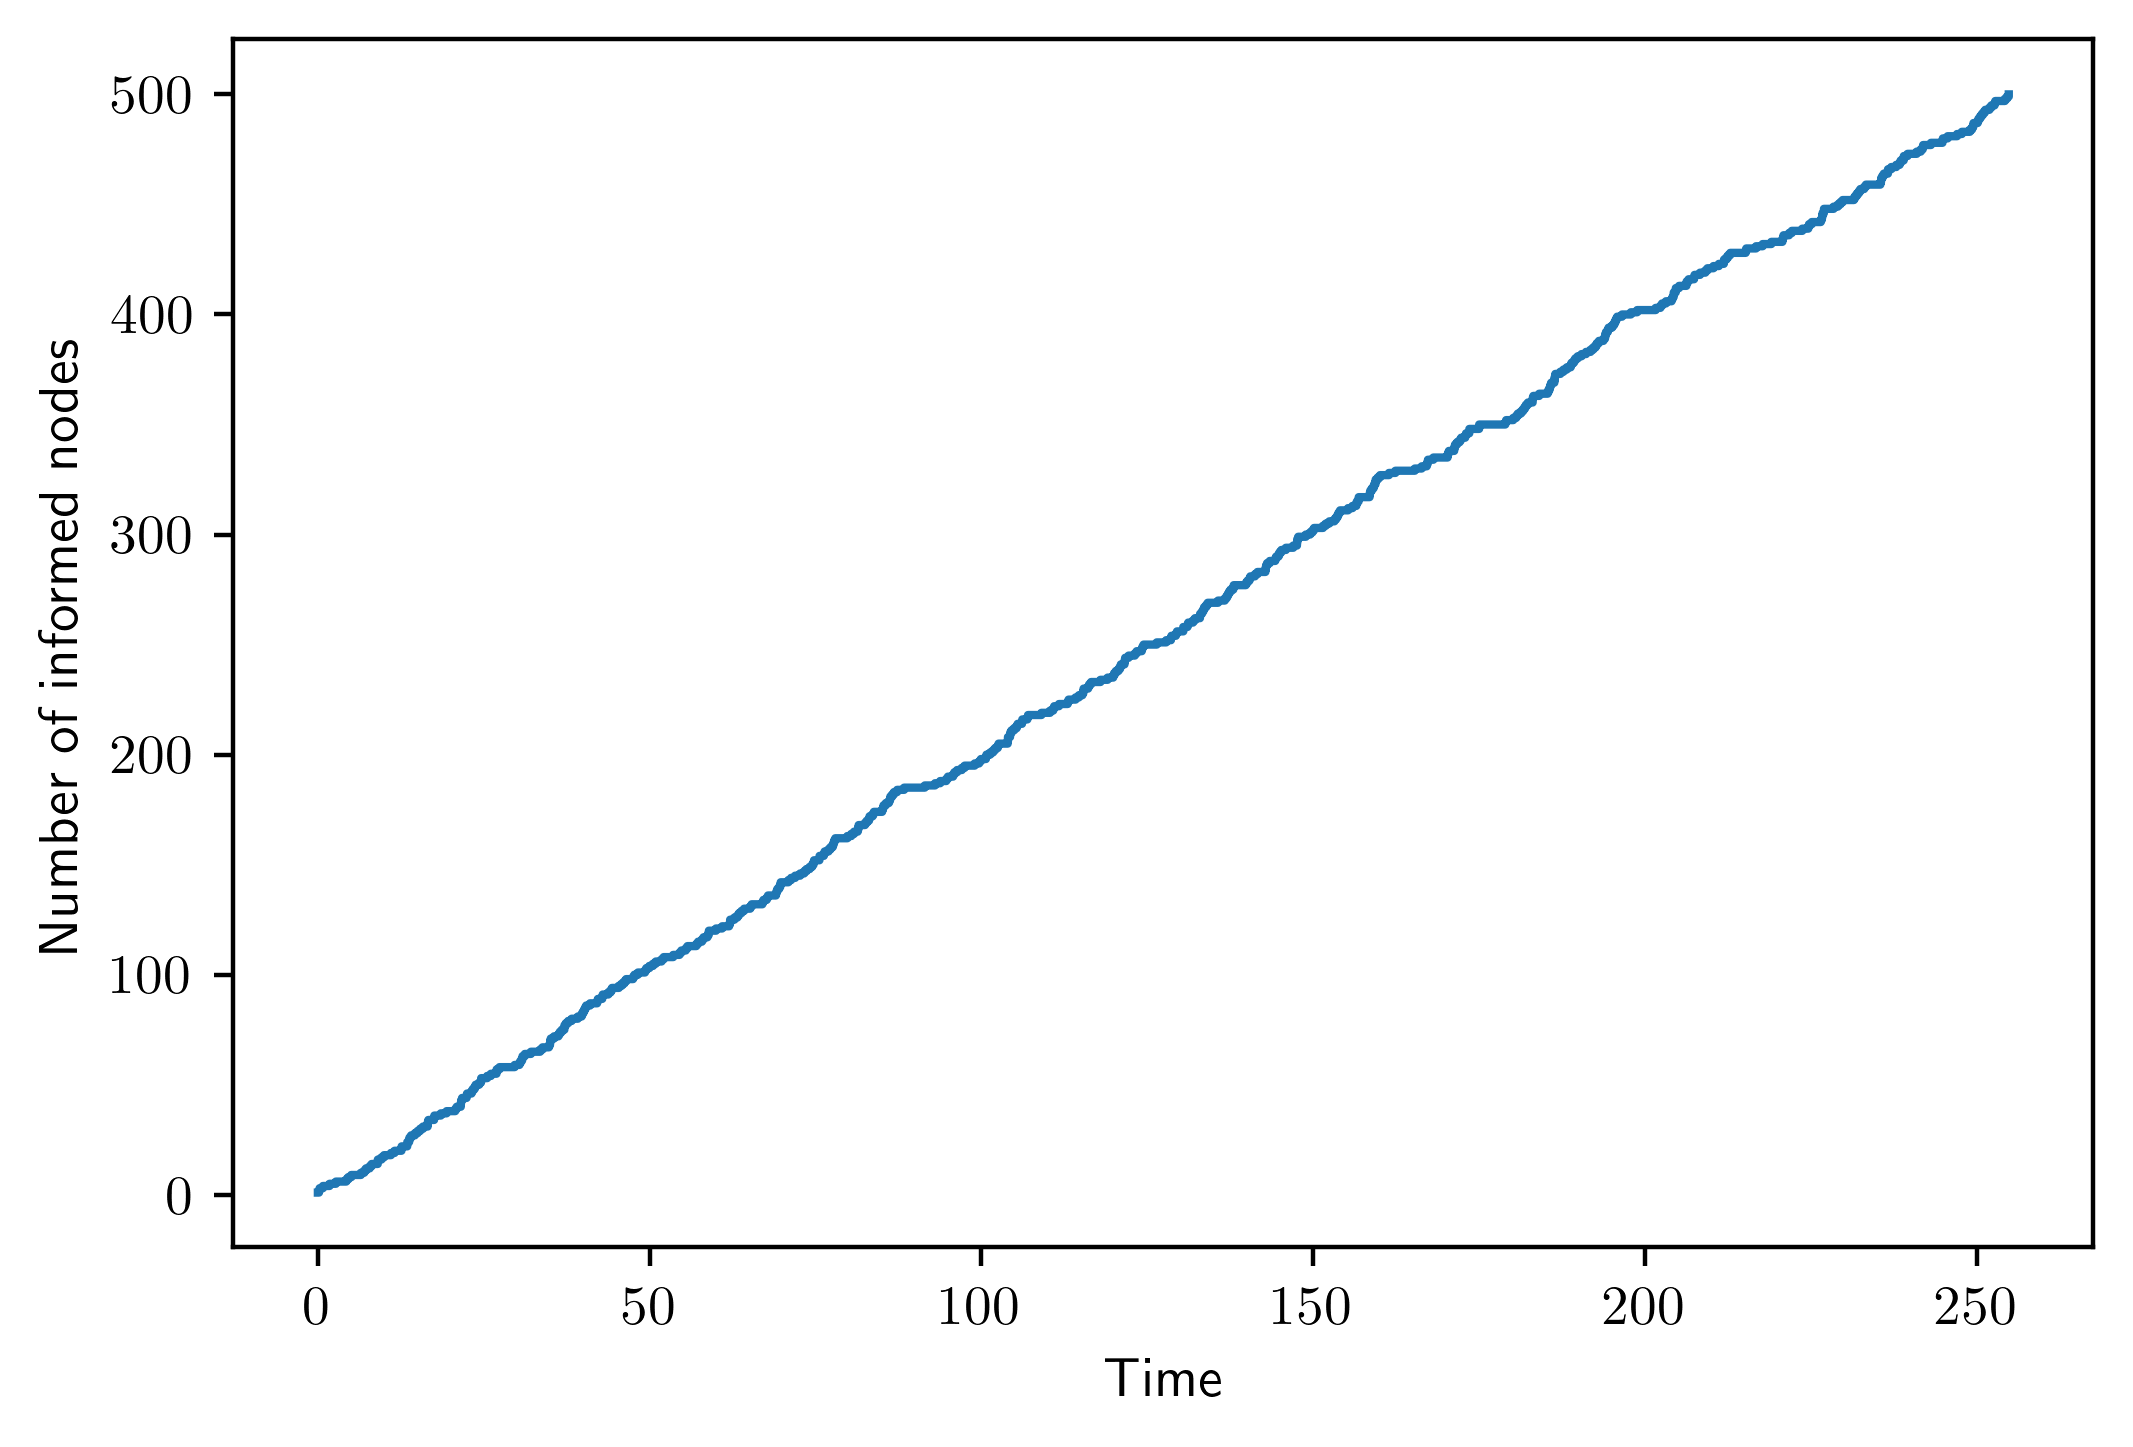
\includegraphics[width=\textwidth]{./figures/static_ring_informed_node_growth.png}
	\caption{Simulated informed node growth over time in the Static Ring Network}
	\label{fig:staticRingInformedNodeGrowth}
\end{figure}

Figure \ref{fig:staticRingInformedNodeGrowth} shows the number of informed nodes at each time during a rumour spread simulation on the Static Ring Network with 500 nodes. Notice that the rate at which the number of informed nodes increases is constant, since at all times there are exactly 2 active edges capable of spreading the rumour.

\begin{figure}[h]
	\centering
	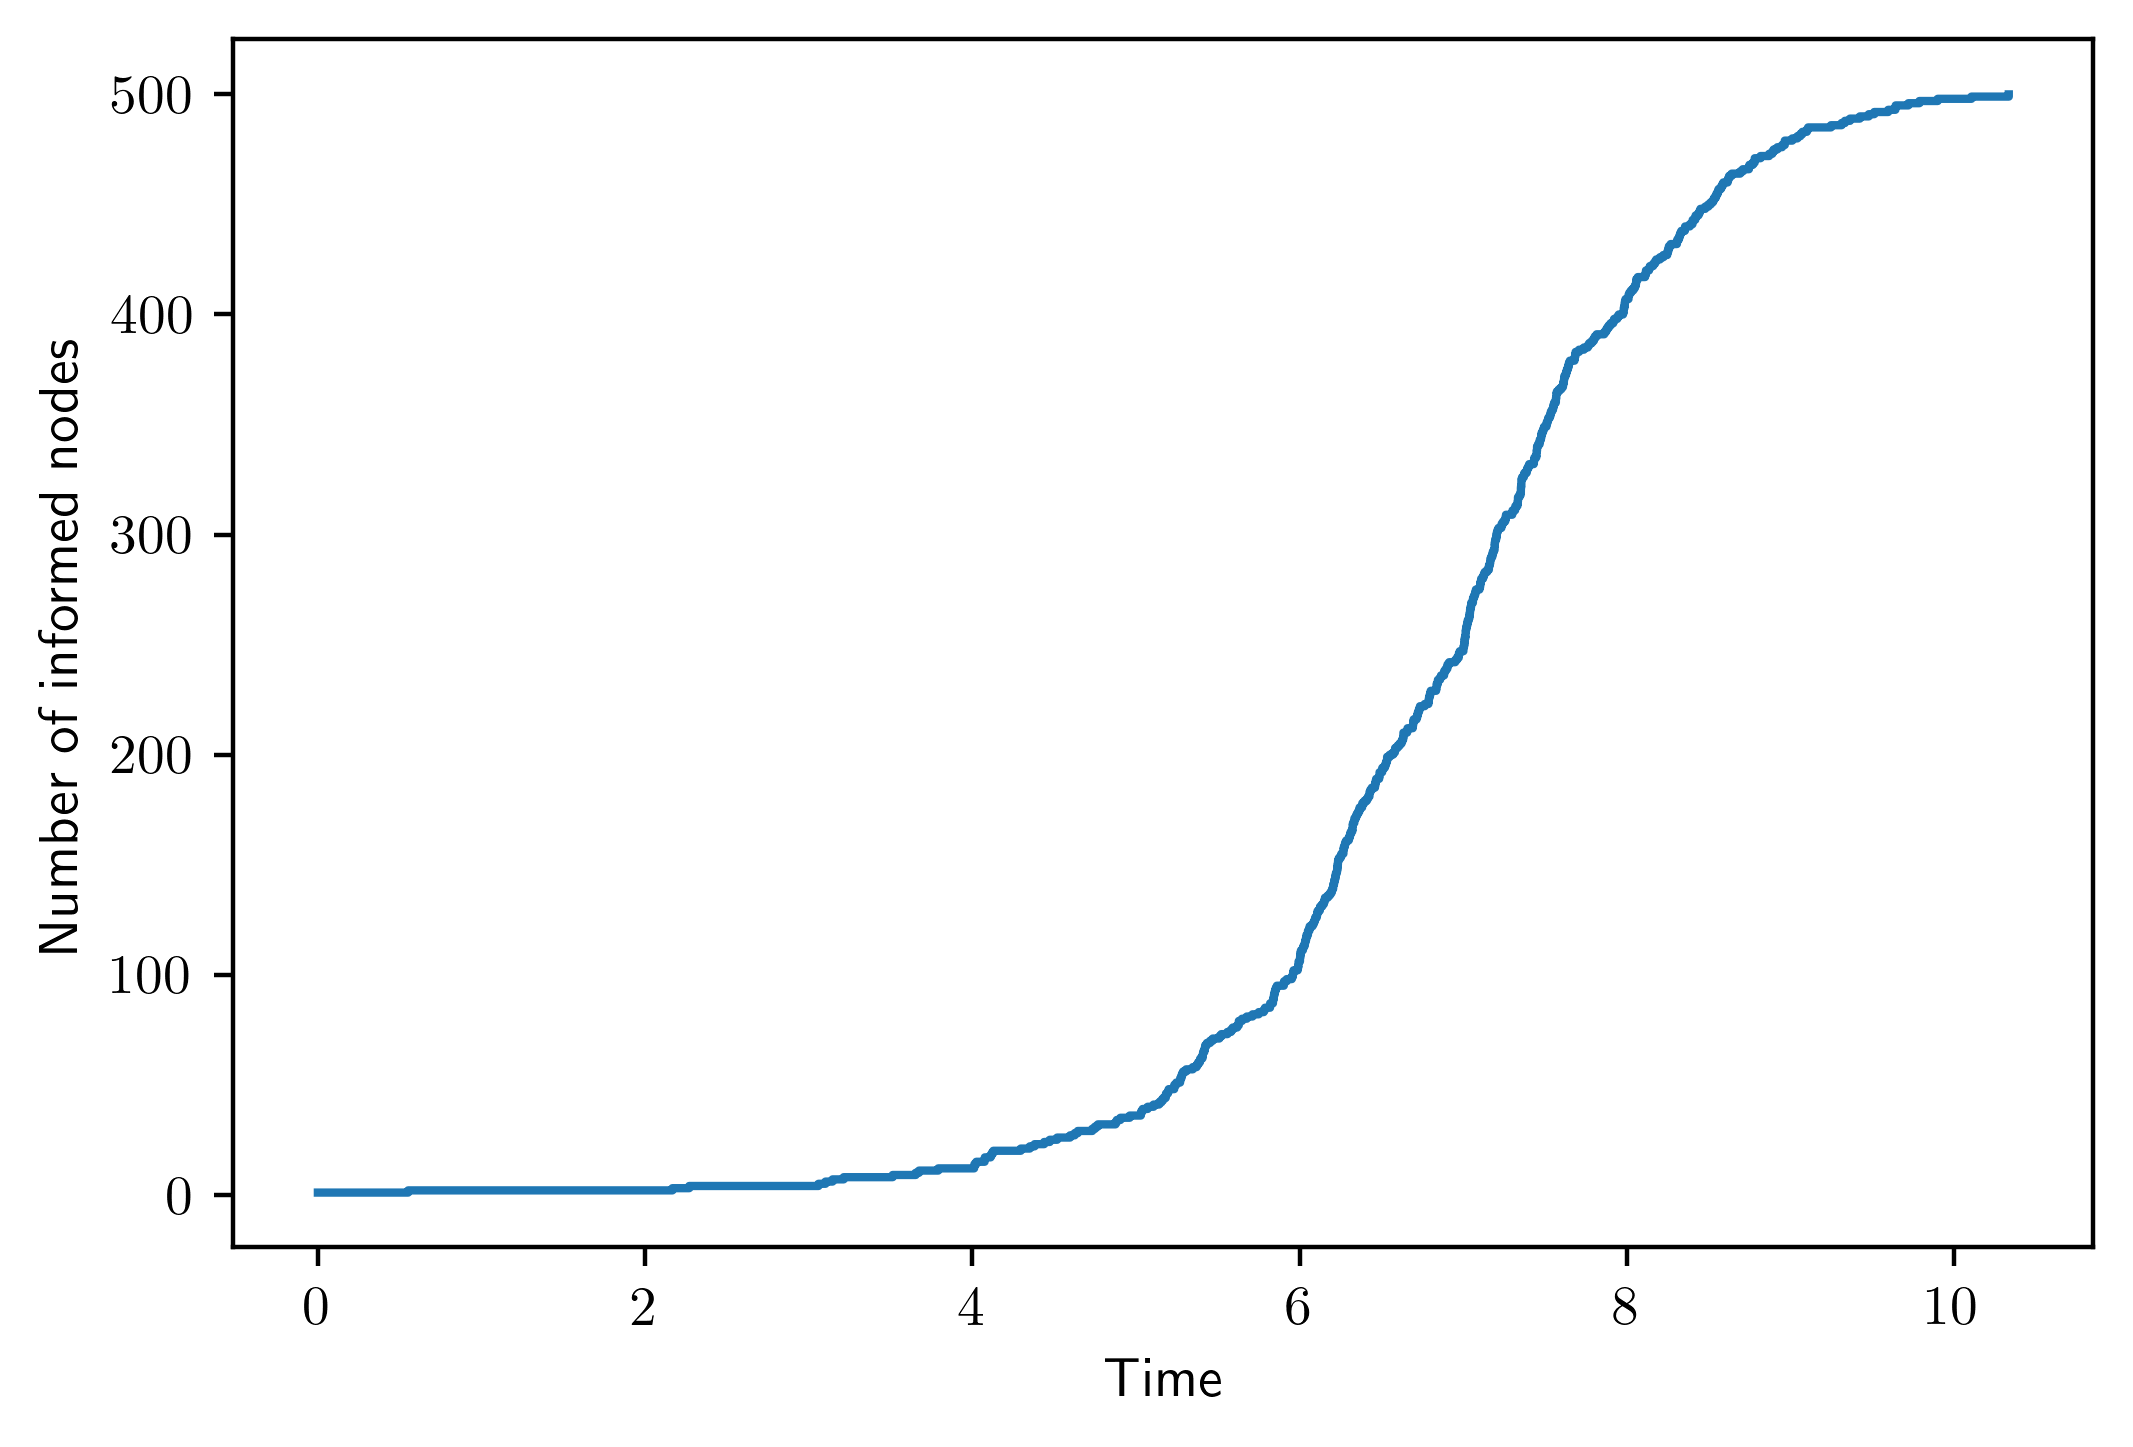
\includegraphics[width=\textwidth]{./figures/shuffled_ring_informed_node_growth.png}
	\caption{Simulated informed node growth over time in the Shuffled Ring Network}
	\label{fig:shuffledRingInformedNodeGrowth}
\end{figure}

Figure \ref{fig:shuffledRingInformedNodeGrowth} is a similar plot for a rumour spread on the Shuffled Ring Network. In this figure we note that the rate at which the number of informed nodes increases varies over time. In the first 3 rounds there are few informed nodes and only 3 opportunities for shuffling, hence the number of active edges is still close to 2. This is reflected in Figure \ref{fig:shuffledRingInformedNodeGrowth} by the initial slow growth in the number of informed nodes. However, after round 4 we see a rapid increase in the rate at which nodes are informed of the rumour, since there are a sufficient number of informed nodes for the shuffling to scatter informed nodes all around the ring, adding many active edges. 
As the network becomes saturated with informed nodes around time 7, the number of active edges begins to decrease as it becomes more likely that informed nodes will still be adjacent to other informed nodes after shuffling. Hence, in Figure \ref{fig:shuffledRingInformedNodeGrowth}, we see the rate of growth begins to decrease.

% MAYBE: Talk about branching process
% This growth is similar to a branching process, where each set of contiguous informed nodes (the parent) has a probability of being split into multiple contiguous sets (the children). In this process the offspring distribution would change over time as the network becomes saturated. An interesting area for further study could be fully characterising this growth as a branching process.

Note that since Algorithm \ref{NodeCentricAsyncAlgorithm} is a random process, the individual simulations analysed in Figures \ref{fig:staticRingInformedNodeGrowth} and \ref{fig:shuffledRingInformedNodeGrowth} are not necessarily characteristic of how the rumour spreads on each network. However, after running the simulations multiple times, we see the same general structures we have discussed in both plots, hence these displays are useful illustrations.

We now return to the question posed in Section \ref{section:shuffledRingAsyncApplication} - why is the bound given by Theorem \ref{theorem:AsyncUpperBound} weak for the Shuffled Ring? We saw in the proof of Theorem \ref{theorem:staticRingAsyncBound} that the $\mathcal{O}(n \log n)$ bound must hold w.h.p for both the Static Ring and Shuffled Ring, since they are isomorphic. However, we have seen from simulations that the spreading time of the Static ring grows like $\mathcal{O}(n)$, so our bound for both the Static Ring and Shuffled Ring can be no better than $\mathcal{O}(n)$. 

We can interpret the Static Ring as a version of the Shuffled Ring in which the nodes have been relabelled. This example shows that such a renaming has no effect on the bound, but has a significant impact on the spreading time, hence the bound must accommodate for the network with the worse spreading time. We refer to such a network as `adversarial', in the sense that it is the network which aims to slow the spread of the rumour by relabelling nodes. This example demonstrates a limitation of the bound: given a network, the bound can be no better than the spreading time of the corresponding adversarial network (the isomorphic network with the slowest spreading time).

For example, all other networks isomorphic but not equal to the Static Ring Network (such as the Shuffle Ring Network) involve some relabelling of nodes between rounds, which could introduce additional active edges. Thus, the Static Ring minimises the number of active edges at all time steps so is in fact the adversarial network for the Shuffled Ring Network. 

In conclusion, we have seen in this section that although sometimes the bound is nearly tight, frequently it is not. After studying the behaviour of rumour spreading on isomorphic ring networks, we also saw that adversarial networks with larger spreading times than their isomorphic networks weaken the bound for these other networks. In this example we saw that the bound was only a factor of $\mathcal{O}(\log n)$ worse than the best possible bound in the adversarial case. But are there other adversarial networks for which the bound is almost tight? And is the adversarial network always the static equivalent of a given network? We investigate these questions in Chapter \ref{chapter:asyncBoundTight}.